\chapter{結果}
本章では,波の各性質をプログラムによって視覚化した実行結果を記述する.いずれのプログラムもJavaScriptへ変換可能であり,Webブラウザ上で動作させることが可能である.

\section{円形波の位相変位を視覚化したプログラム}
図\ref{fig:4wave}は指定した複数の点源から生成される円形波の位相変位をシミュレーションし,視覚化を行うプログラムである.
このプログラムにはdrawモードとcheckモードという2つのモードが実装されており,drawモードからcheckモードに移行するにはCキー(checkの頭文字).checkモードからdrawモードに移行するときはDキー(drawの頭文字)を押せばよい.


\begin{figure}[htbp]
 \begin{center}
  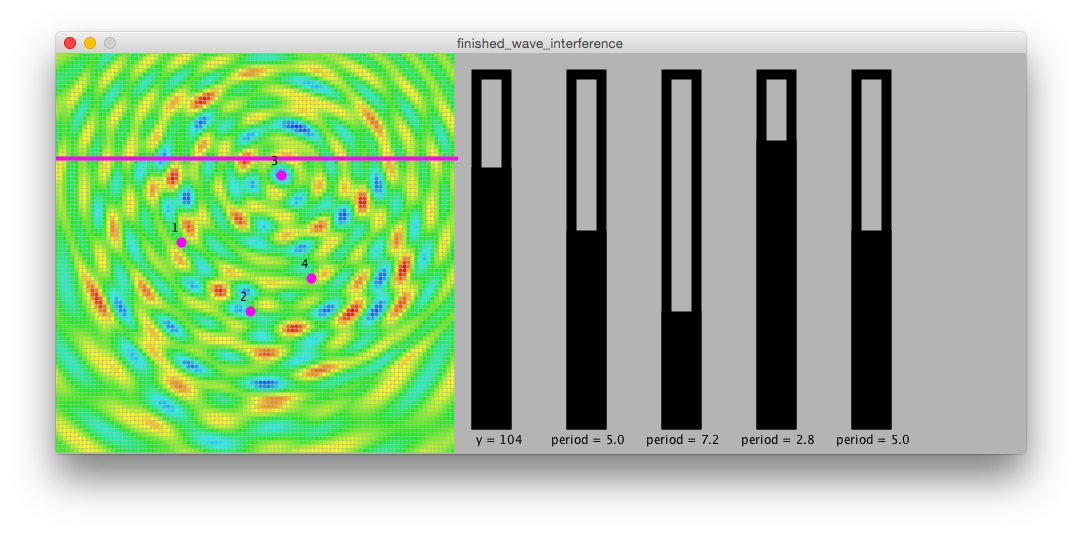
\includegraphics[width=\linewidth]{../result/4wave.png}
 \end{center}
 \caption{波の位相変位を視覚化したプログラムの画面.}
 \label{fig:4wave}
\end{figure}






\subsection{drawモード}
このモードは波源から生じる円形波を描写するモードである. プログラム起動時の画面が図\ref{fig:0wave}である.
\begin{figure}[htbp]
 \begin{center}
  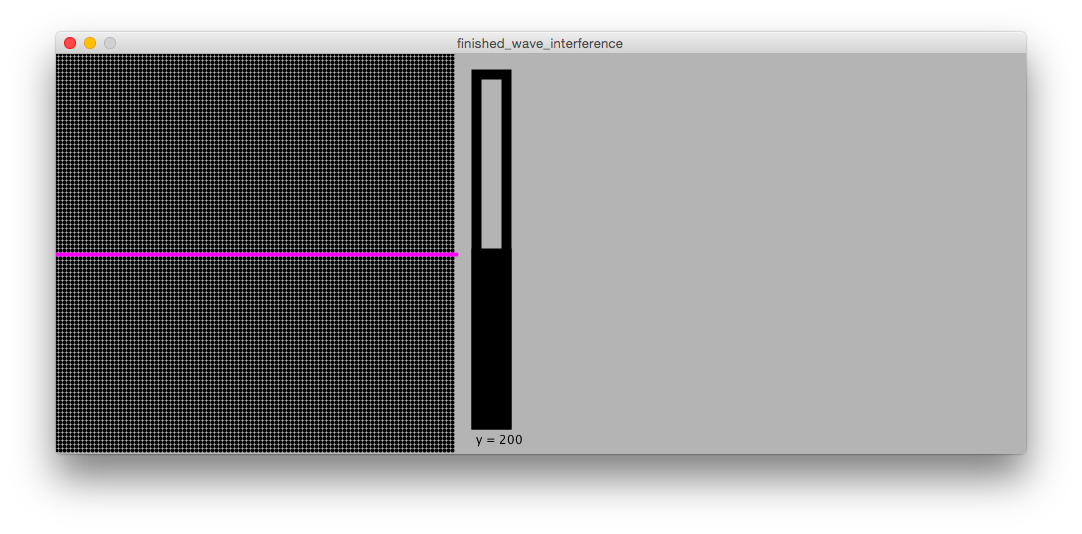
\includegraphics[width=\linewidth]{../result/0wave.png}
 \end{center}
 \caption{プログラム起動時の画面.}
 \label{fig:0wave}
\end{figure}

画面左側の黒い領域が波を描写する領域,画面右側にはcheckモードで確認するy座標の位置を操作できるスライダーが配置されている(いきなりスライダーと言っていいのか?). 
図\ref{fig:0wave}の状態で黒い領域上のいずれかの場所をクリックすると,クリックされた座標に波源が生成される.波源が生成されたあと,画面右側にはその波源の周期を変更できるスライダーが生成される.

図\ref{fig:wave}は1つの波源を生成した後,周期をスライダーによって変更した様子である.
\begin{figure}[htbp]
 \begin{center}
  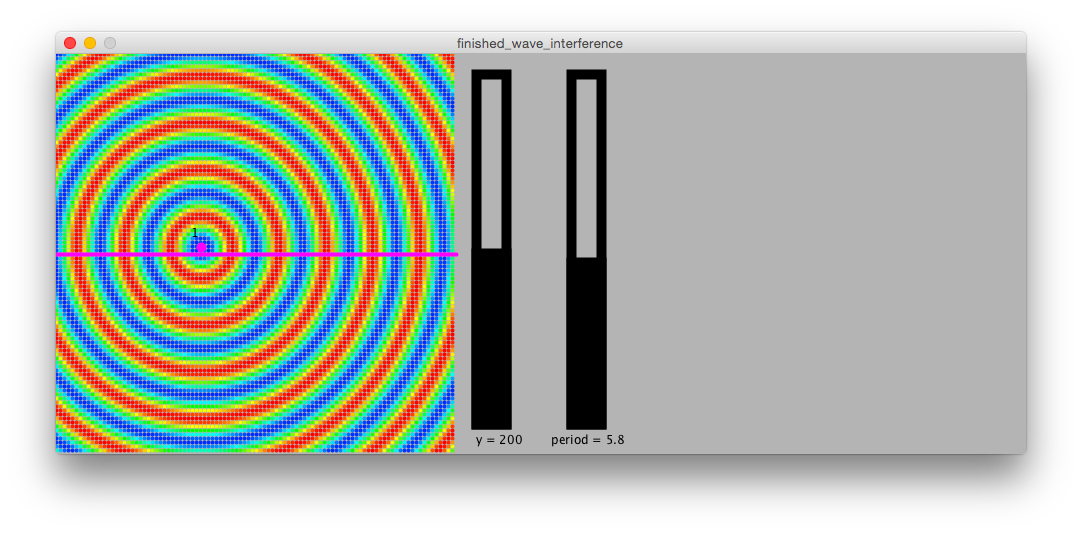
\includegraphics[width=\linewidth]{../result/wave.png}
 \end{center}
 \caption{1つの波の周期をスライダーで変更した画面.}
 \label{fig:wave}
\end{figure}

\newpage
スライダーが周期を変更できる状態で
Lキー(lambdaの頭文字)を押すと,図\ref{fig:wavechangelambda}のように波の波長を変更できるスライダーに変化する.周期を変更するスライダーに戻したい場合はPキー(periodの頭文字)を押せばよい.

\begin{figure}[htbp]
 \begin{center}
  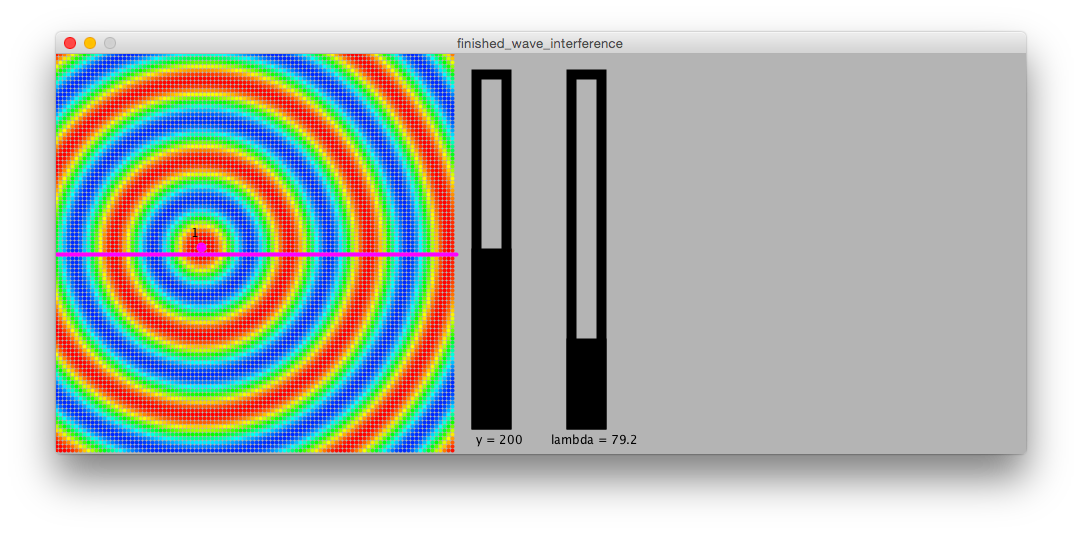
\includegraphics[width=\linewidth]{../result/wavechangelambda.png}
 \end{center}
 \caption{波長を変更できるスライダーに変化させた時の画面.}
 \label{fig:wavechangelambda}
\end{figure}

波源は図\ref{fig:5wave}のように5個まで生成できる.

\begin{figure}[htbp]
 \begin{center}
  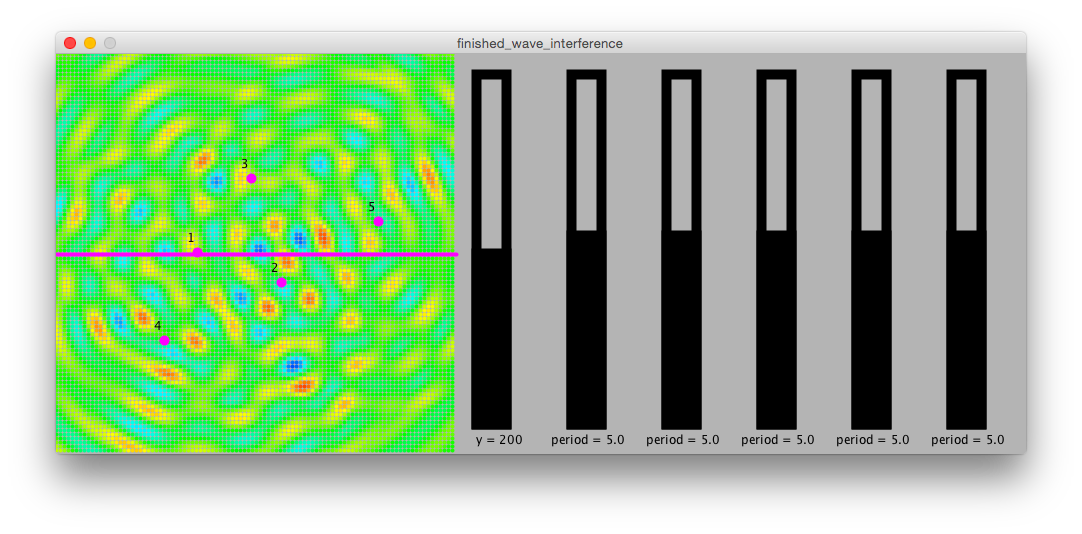
\includegraphics[width=\linewidth]{../result/5wave.png}
 \end{center}
 \caption{波源を5個生成した時の画面.}
 \label{fig:5wave}
\end{figure}

\newpage
\subsection{checkモード}
このモードはdrawモードに描写されている赤い線上の位相変位をリアルタイムに視覚化するモードである.同時刻,同座標で周期,波長が同一な波を生成し,波を生成して360フレーム目の状態をdrawモード,checkモードでそれぞれ描写したのが図\ref{fig:compare}(\subref{drawmode}),(\subref{checkmode})である.(ほんまに一致しているか先生に見てもらう)


\begin{figure}[htbp]
\begin{minipage}[b]{1.0\linewidth}
\centering
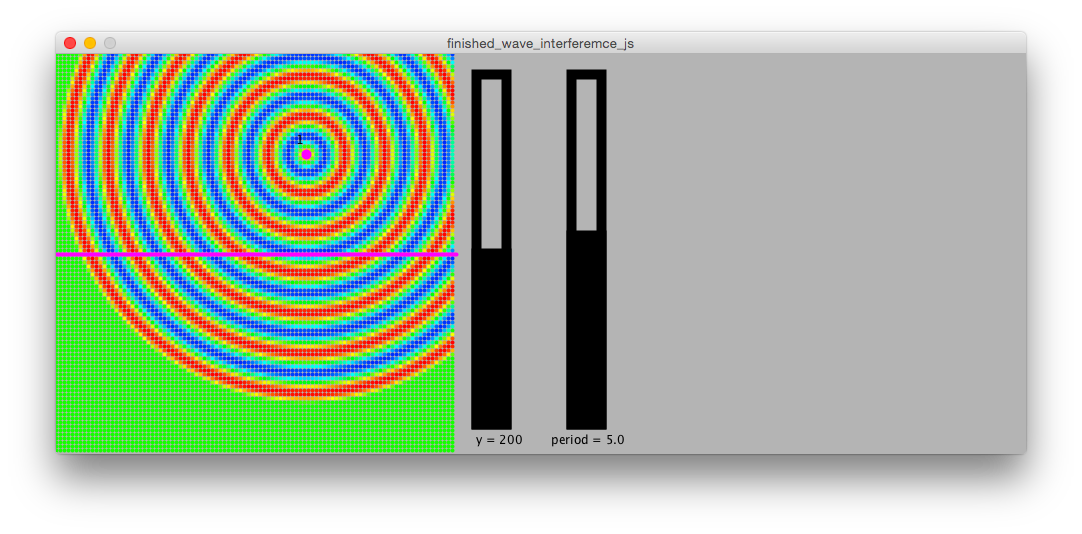
\includegraphics[keepaspectratio, scale=0.40]
  {../result/drawmode.png}
 \subcaption{drawモード.}\label{drawmode}
 \end{minipage}
 
\begin{minipage}[b]{1.0\linewidth}
\centering
  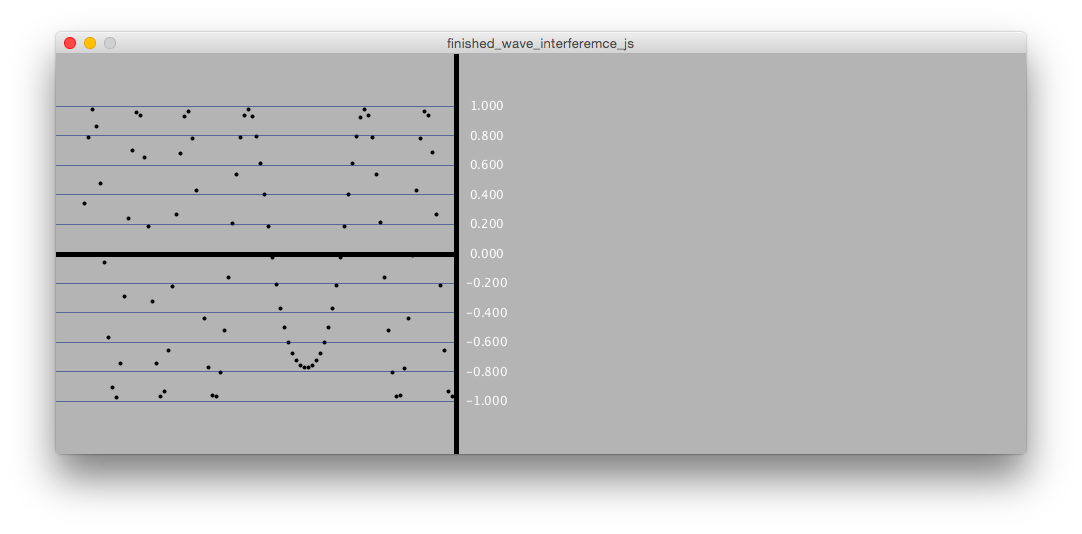
\includegraphics[keepaspectratio, scale=0.40]
  {../result/checkmode.png}
 \subcaption{checkモード.}\label{checkmode}
 \end{minipage}
  
  \caption{周期5.0,波長40.0の波が生成されてから360フレーム目のdrawモード,checkモードの画面.}
 \label{fig:compare}
\end{figure}



\newpage
\section{波の回折現象を視覚化したプログラム}
\section{波の反射を視覚化したプログラム}
出来なかった理由はプログラム解説の章で解説していいのか?
\section{波の屈折を視覚化したプログラム}























\begin{comment}

%図\ref{fig:MDprogram}は本研究で作成したVerlet法とLennard-Jonesポテンシャルを用いて粒子の振る舞いをシミュレーションし,視覚化を行うプログラムである.
%Processingで作成しているが,JavaScriptへ変換する事によってWebブラウザ上で動作させる事が可能である.
%左の枠内に複数の粒子モデルが描画され,それらが枠内を動き回る.また,粒子の色を速度によって青から赤に変化させてエネルギーの推移をわかりやすくし,マウスカーソルで粒子をクリックしドラッグする\chapter{結果}
本章では,波の各性質をプログラムによって視覚化した実行結果を記述する.いずれのプログラムもJavaScriptへ変換可能であり,Webブラウザ上で動作させることが可能である.

\section{円形波の位相変位を視覚化したプログラム}
図\ref{fig:4wave}は指定した複数の点源から生成される円形波の位相変位をシミュレーションし,視覚化を行うプログラムである.
このプログラムにはdrawモードとcheckモードという2つのモードが実装されており,drawモードからcheckモードに移行するにはCキー(checkの頭文字).checkモードからdrawモードに移行するときはDキー(drawの頭文字)を押せばよい.


\begin{figure}[htbp]
 \begin{center}
  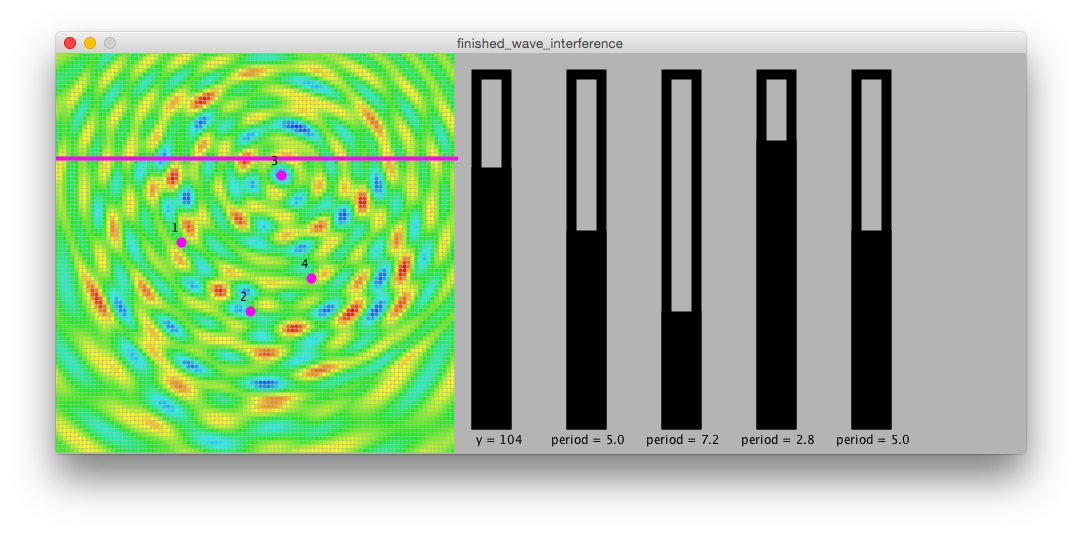
\includegraphics[width=\linewidth]{../result/4wave.png}
 \end{center}
 \caption{波の位相変位を視覚化したプログラムの画面.}
 \label{fig:4wave}
\end{figure}






\subsection{drawモード}
このモードは波源から生じる円形波を描写するモードである. プログラム起動時の画面が図\ref{fig:0wave}である.
\begin{figure}[htbp]
 \begin{center}
  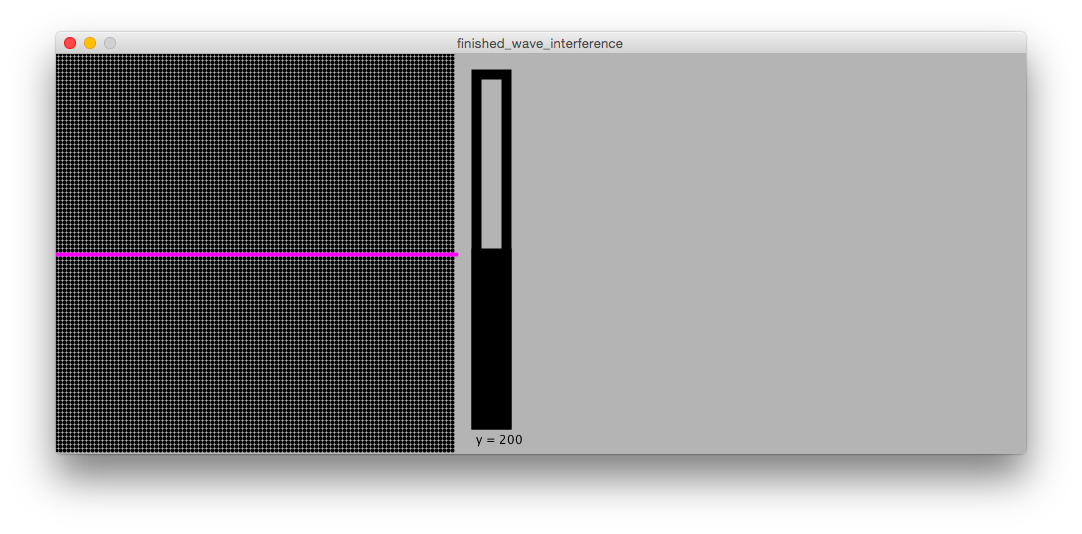
\includegraphics[width=\linewidth]{../result/0wave.png}
 \end{center}
 \caption{プログラム起動時の画面.}
 \label{fig:0wave}
\end{figure}

画面左側の黒い領域が波を描写する領域,画面右側にはcheckモードで確認するy座標の位置を操作できるスライダーが配置されている(いきなりスライダーと言っていいのか?). 
図\ref{fig:0wave}の状態で黒い領域上のいずれかの場所をクリックすると,クリックされた座標に波源が生成される.波源が生成されたあと,画面右側にはその波源の周期を変更できるスライダーが生成される.

図\ref{fig:wave}は1つの波源を生成した後,周期をスライダーによって変更した様子である.
\begin{figure}[htbp]
 \begin{center}
  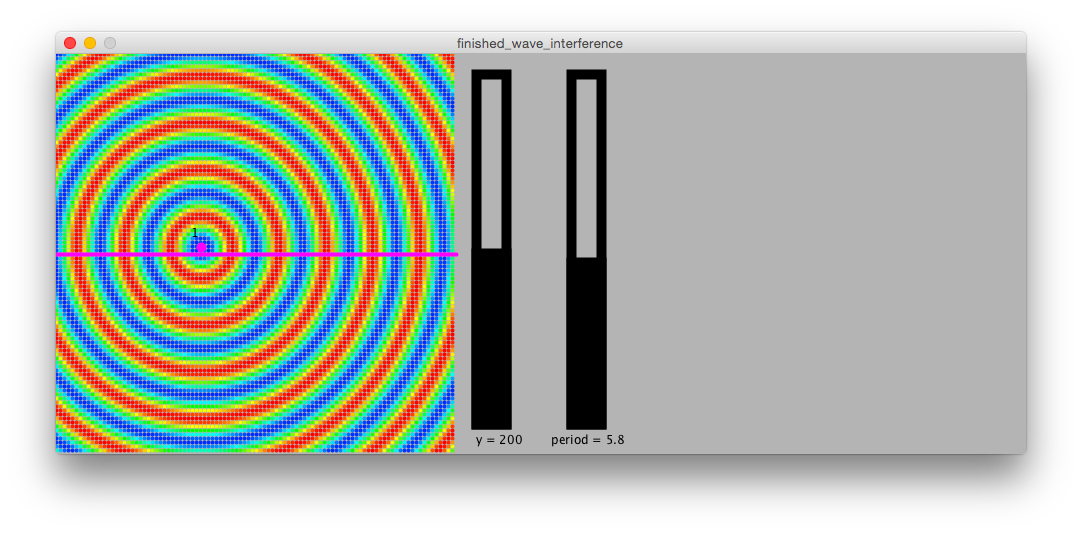
\includegraphics[width=\linewidth]{../result/wave.png}
 \end{center}
 \caption{1つの波の周期をスライダーで変更した画面.}
 \label{fig:wave}
\end{figure}

\newpage
スライダーが周期を変更できる状態で
Lキー(lambdaの頭文字)を押すと,図\ref{fig:wavechangelambda}のように波の波長を変更できるスライダーに変化する.周期を変更するスライダーに戻したい場合はPキー(periodの頭文字)を押せばよい.

\begin{figure}[htbp]
 \begin{center}
  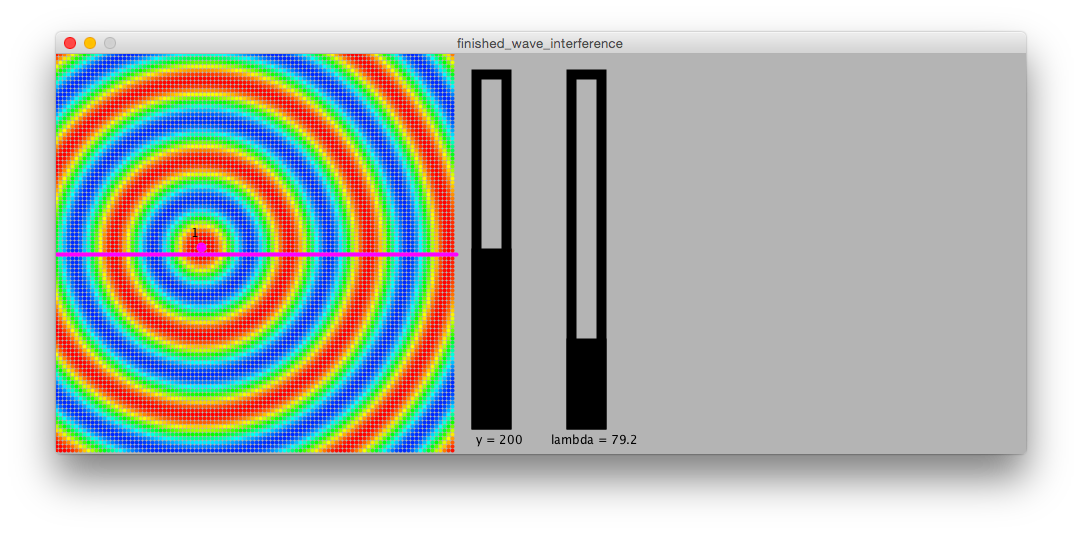
\includegraphics[width=\linewidth]{../result/wavechangelambda.png}
 \end{center}
 \caption{波長を変更できるスライダーに変化させた時の画面.}
 \label{fig:wavechangelambda}
\end{figure}

波源は図\ref{fig:5wave}のように5個まで生成できる.

\begin{figure}[htbp]
 \begin{center}
  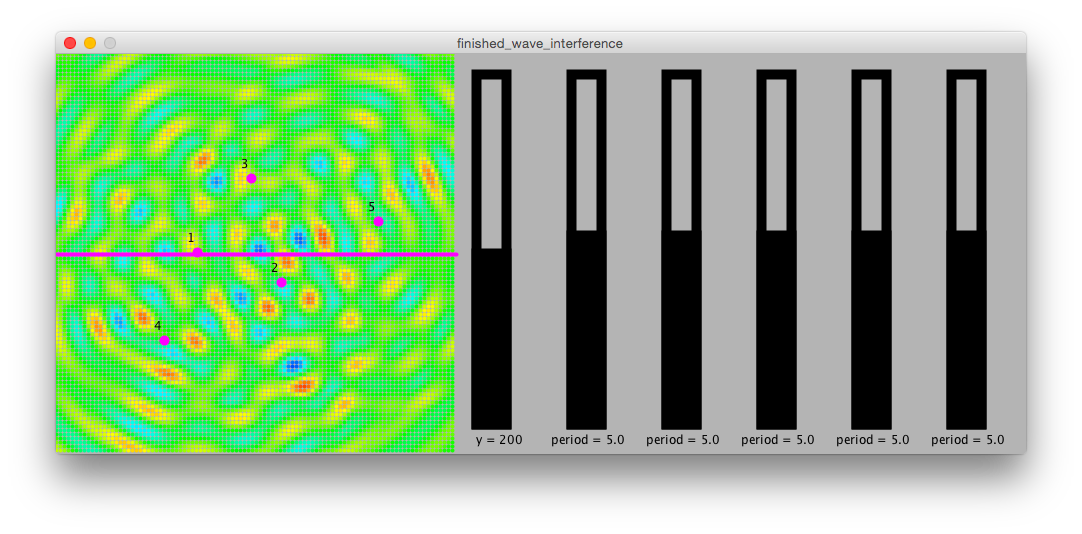
\includegraphics[width=\linewidth]{../result/5wave.png}
 \end{center}
 \caption{波源を5個生成した時の画面.}
 \label{fig:5wave}
\end{figure}

\newpage
\subsection{checkモード}
このモードはdrawモードに描写されている赤い線上の位相変位をリアルタイムに視覚化するモードである.同時刻,同座標で周期,波長が同一な波を生成し,波を生成して360フレーム目の状態をdrawモード,checkモードでそれぞれ描写したのが図\ref{fig:compare}(\subref{drawmode}),(\subref{checkmode})である.(ほんまに一致しているか先生に見てもらう)


\begin{figure}[htbp]
\begin{minipage}[b]{1.0\linewidth}
\centering
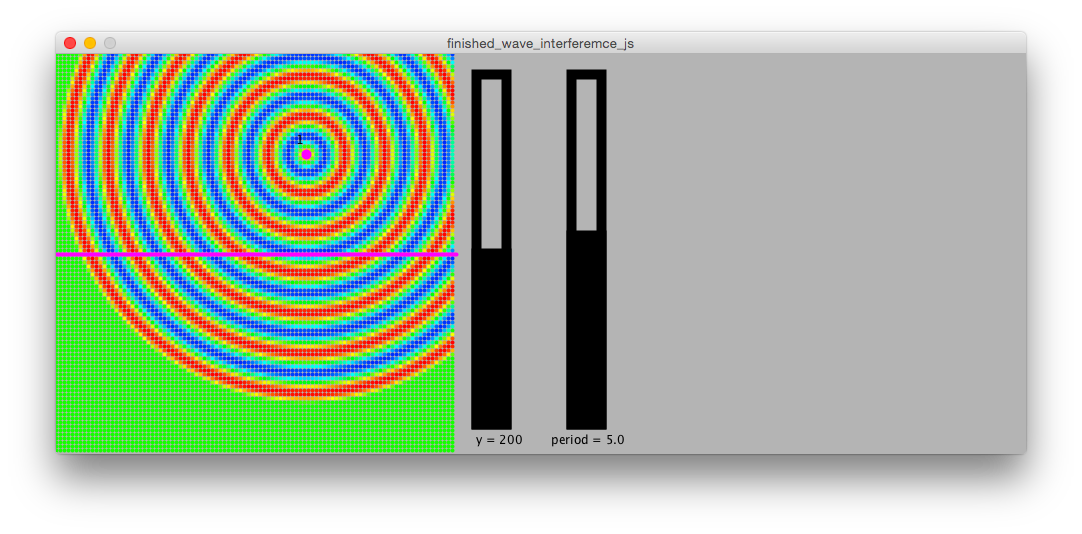
\includegraphics[keepaspectratio, scale=0.40]
  {../result/drawmode.png}
 \subcaption{drawモード.}\label{drawmode}
 \end{minipage}
 
\begin{minipage}[b]{1.0\linewidth}
\centering
  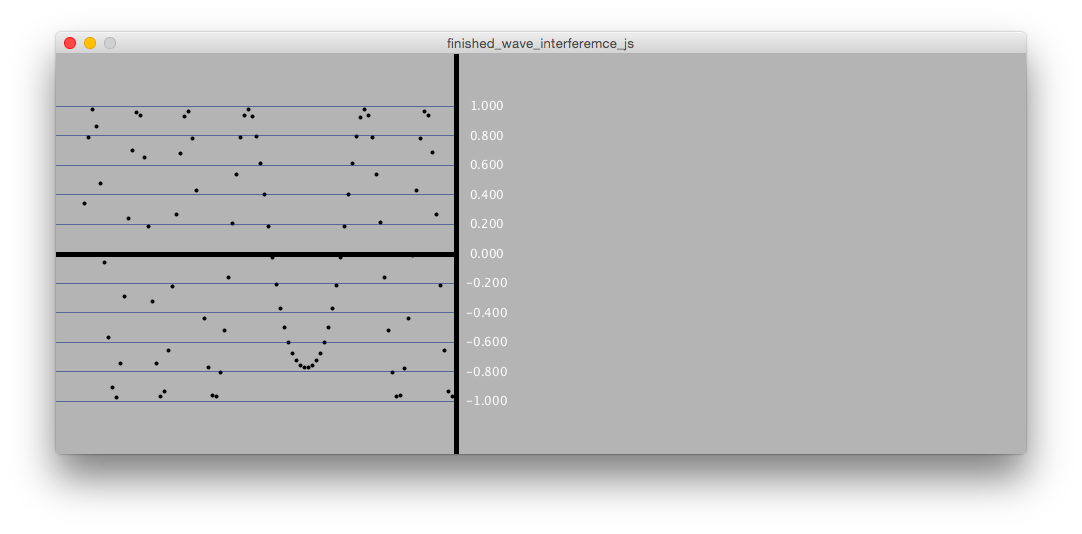
\includegraphics[keepaspectratio, scale=0.40]
  {../result/checkmode.png}
 \subcaption{checkモード.}\label{checkmode}
 \end{minipage}
  
  \caption{周期5.0,波長40.0の波が生成されてから360フレーム目のdrawモード,checkモードの画面.}
 \label{fig:compare}
\end{figure}



\newpage
\section{波の回折現象を視覚化したプログラム}
\section{波の反射を視覚化したプログラム}
出来なかった理由はプログラム解説の章で解説していいのか?
\section{波の屈折を視覚化したプログラム}























\begin{comment}

%図\ref{fig:MDprogram}は本研究で作成したVerlet法とLennard-Jonesポテンシャルを用いて粒子の振る舞いをシミュレーションし,視覚化を行うプログラムである.
%Processingで作成しているが,JavaScriptへ変換する事によってWebブラウザ上で動作させる事が可能である.
%左の枠内に複数の粒子モデルが描画され,それらが枠内を動き回る.また,粒子の色を速度によって青から赤に変化させてエネルギーの推移をわかりやすくし,マウスカーソルで粒子をクリックしドラッグする\chapter{結果}
本章では,波の各性質をプログラムによって視覚化した実行結果を記述する.いずれのプログラムもJavaScriptへ変換可能であり,Webブラウザ上で動作させることが可能である.

\section{円形波の位相変位を視覚化したプログラム}
図\ref{fig:4wave}は指定した複数の点源から生成される円形波の位相変位をシミュレーションし,視覚化を行うプログラムである.
このプログラムにはdrawモードとcheckモードという2つのモードが実装されており,drawモードからcheckモードに移行するにはCキー(checkの頭文字).checkモードからdrawモードに移行するときはDキー(drawの頭文字)を押せばよい.


\begin{figure}[htbp]
 \begin{center}
  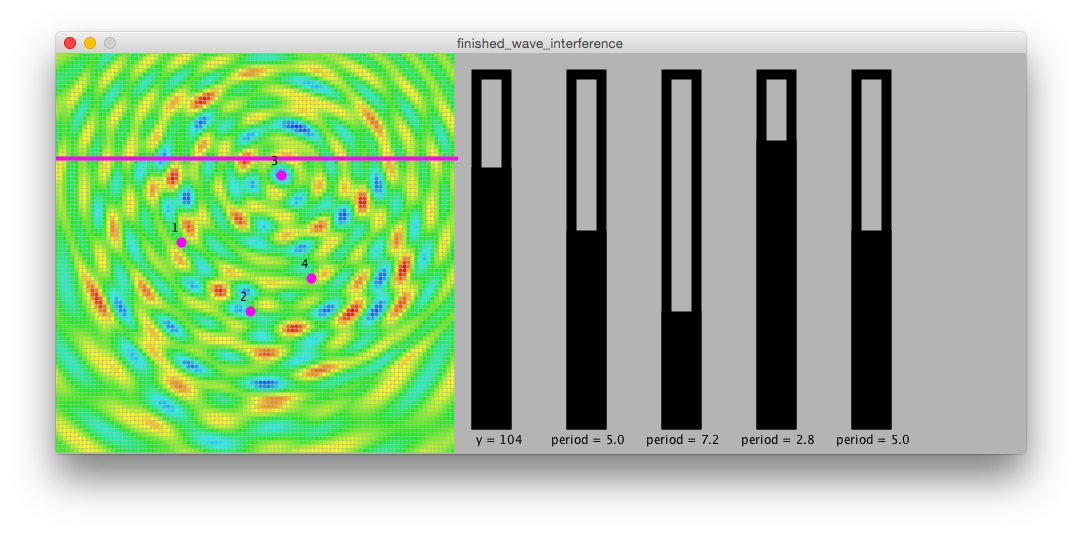
\includegraphics[width=\linewidth]{../result/4wave.png}
 \end{center}
 \caption{波の位相変位を視覚化したプログラムの画面.}
 \label{fig:4wave}
\end{figure}






\subsection{drawモード}
このモードは波源から生じる円形波を描写するモードである. プログラム起動時の画面が図\ref{fig:0wave}である.
\begin{figure}[htbp]
 \begin{center}
  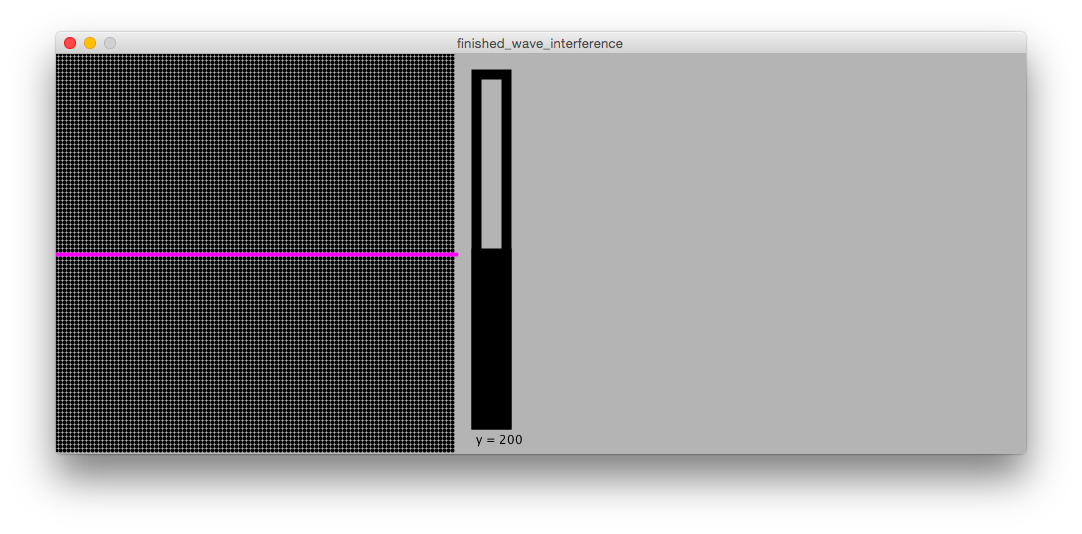
\includegraphics[width=\linewidth]{../result/0wave.png}
 \end{center}
 \caption{プログラム起動時の画面.}
 \label{fig:0wave}
\end{figure}

画面左側の黒い領域が波を描写する領域,画面右側にはcheckモードで確認するy座標の位置を操作できるスライダーが配置されている(いきなりスライダーと言っていいのか?). 
図\ref{fig:0wave}の状態で黒い領域上のいずれかの場所をクリックすると,クリックされた座標に波源が生成される.波源が生成されたあと,画面右側にはその波源の周期を変更できるスライダーが生成される.

図\ref{fig:wave}は1つの波源を生成した後,周期をスライダーによって変更した様子である.
\begin{figure}[htbp]
 \begin{center}
  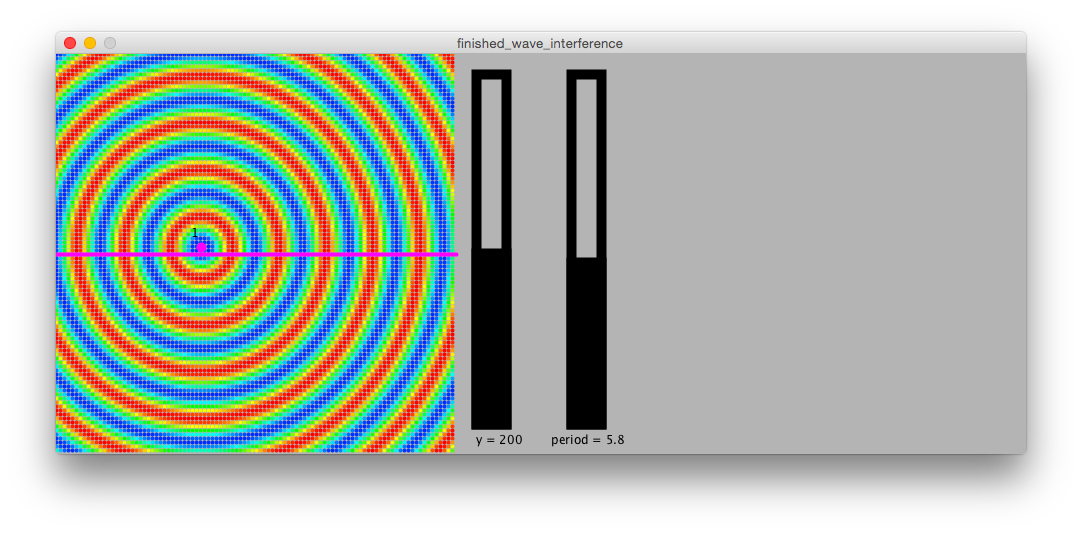
\includegraphics[width=\linewidth]{../result/wave.png}
 \end{center}
 \caption{1つの波の周期をスライダーで変更した画面.}
 \label{fig:wave}
\end{figure}

\newpage
スライダーが周期を変更できる状態で
Lキー(lambdaの頭文字)を押すと,図\ref{fig:wavechangelambda}のように波の波長を変更できるスライダーに変化する.周期を変更するスライダーに戻したい場合はPキー(periodの頭文字)を押せばよい.

\begin{figure}[htbp]
 \begin{center}
  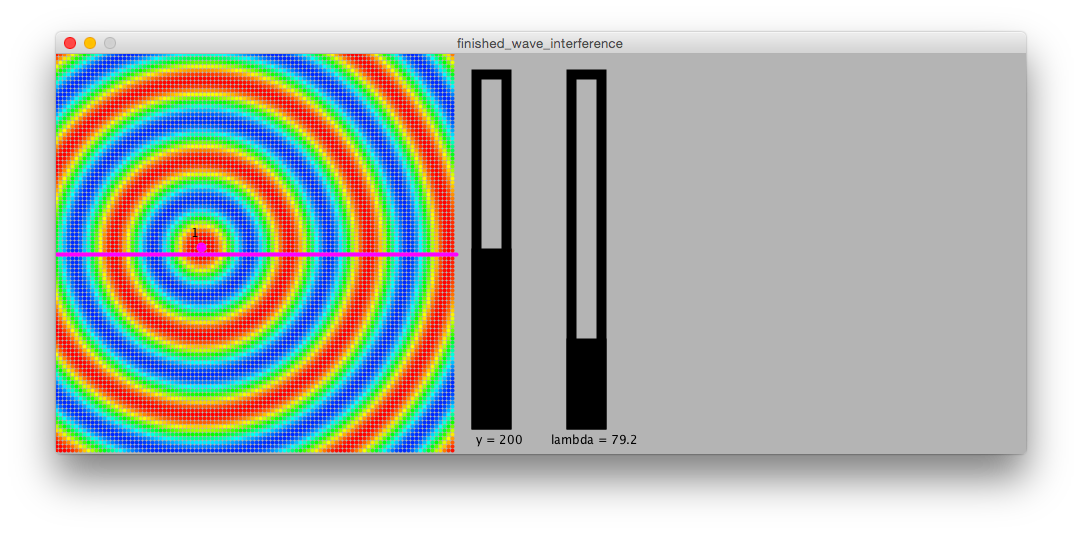
\includegraphics[width=\linewidth]{../result/wavechangelambda.png}
 \end{center}
 \caption{波長を変更できるスライダーに変化させた時の画面.}
 \label{fig:wavechangelambda}
\end{figure}

波源は図\ref{fig:5wave}のように5個まで生成できる.

\begin{figure}[htbp]
 \begin{center}
  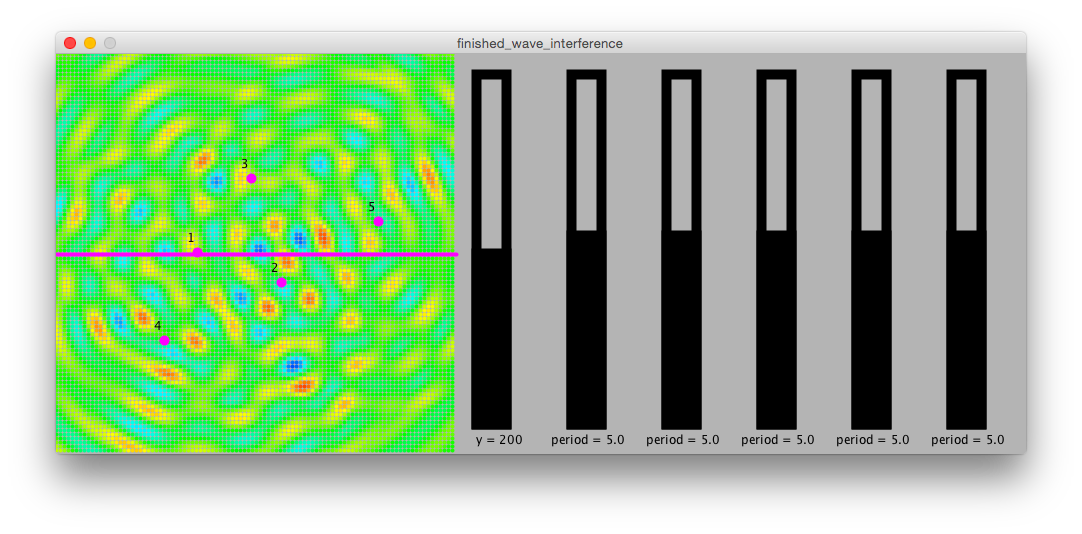
\includegraphics[width=\linewidth]{../result/5wave.png}
 \end{center}
 \caption{波源を5個生成した時の画面.}
 \label{fig:5wave}
\end{figure}

\newpage
\subsection{checkモード}
このモードはdrawモードに描写されている赤い線上の位相変位をリアルタイムに視覚化するモードである.同時刻,同座標で周期,波長が同一な波を生成し,波を生成して360フレーム目の状態をdrawモード,checkモードでそれぞれ描写したのが図\ref{fig:compare}(\subref{drawmode}),(\subref{checkmode})である.(ほんまに一致しているか先生に見てもらう)


\begin{figure}[htbp]
\begin{minipage}[b]{1.0\linewidth}
\centering
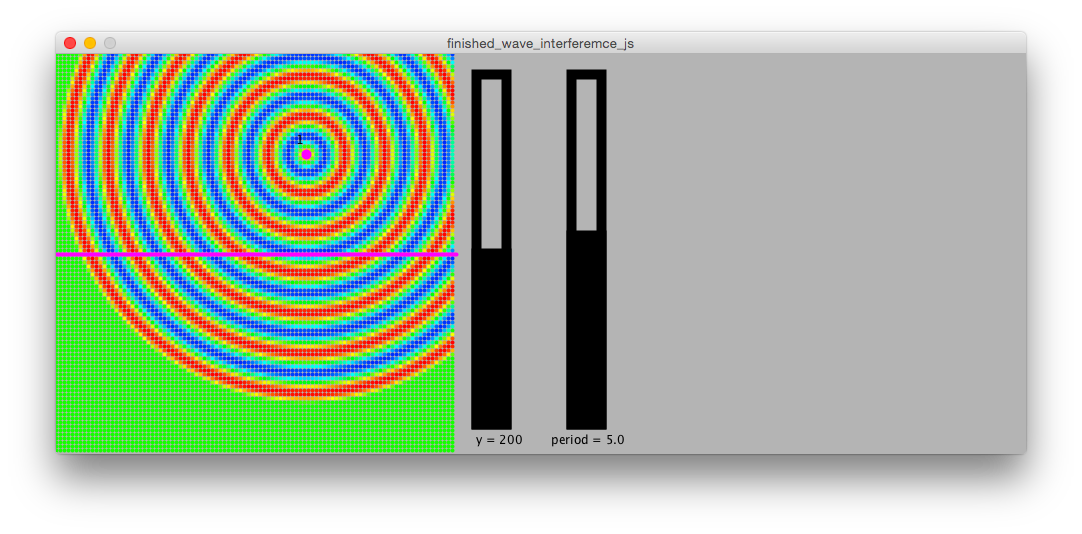
\includegraphics[keepaspectratio, scale=0.40]
  {../result/drawmode.png}
 \subcaption{drawモード.}\label{drawmode}
 \end{minipage}
 
\begin{minipage}[b]{1.0\linewidth}
\centering
  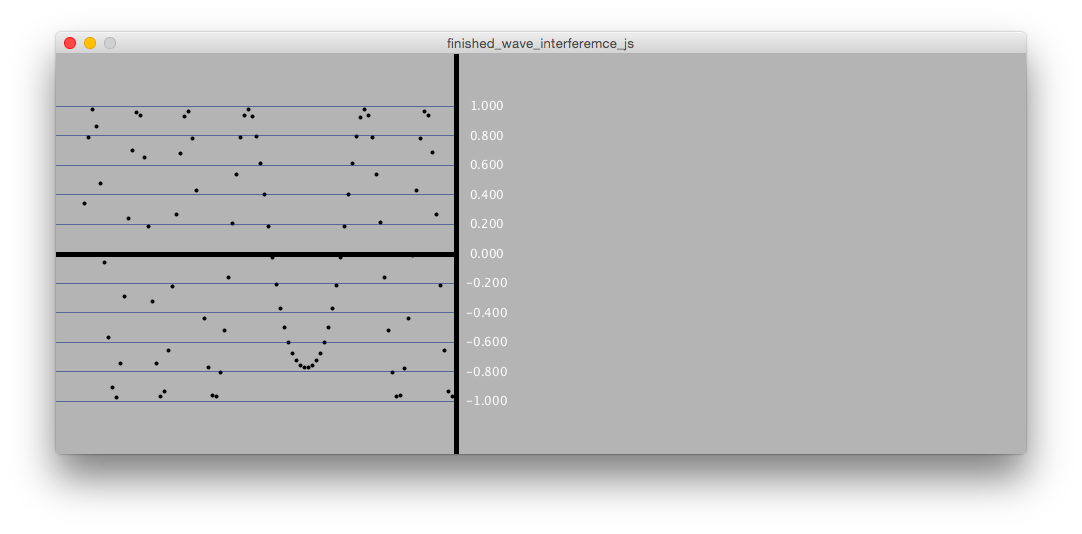
\includegraphics[keepaspectratio, scale=0.40]
  {../result/checkmode.png}
 \subcaption{checkモード.}\label{checkmode}
 \end{minipage}
  
  \caption{周期5.0,波長40.0の波が生成されてから360フレーム目のdrawモード,checkモードの画面.}
 \label{fig:compare}
\end{figure}



\newpage
\section{波の回折現象を視覚化したプログラム}
\section{波の反射を視覚化したプログラム}
出来なかった理由はプログラム解説の章で解説していいのか?
\section{波の屈折を視覚化したプログラム}























\begin{comment}

%図\ref{fig:MDprogram}は本研究で作成したVerlet法とLennard-Jonesポテンシャルを用いて粒子の振る舞いをシミュレーションし,視覚化を行うプログラムである.
%Processingで作成しているが,JavaScriptへ変換する事によってWebブラウザ上で動作させる事が可能である.
%左の枠内に複数の粒子モデルが描画され,それらが枠内を動き回る.また,粒子の色を速度によって青から赤に変化させてエネルギーの推移をわかりやすくし,マウスカーソルで粒子をクリックしドラッグする\chapter{結果}
本章では,波の各性質をプログラムによって視覚化した実行結果を記述する.いずれのプログラムもJavaScriptへ変換可能であり,Webブラウザ上で動作させることが可能である.

\section{円形波の位相変位を視覚化したプログラム}
図\ref{fig:4wave}は指定した複数の点源から生成される円形波の位相変位をシミュレーションし,視覚化を行うプログラムである.
このプログラムにはdrawモードとcheckモードという2つのモードが実装されており,drawモードからcheckモードに移行するにはCキー(checkの頭文字).checkモードからdrawモードに移行するときはDキー(drawの頭文字)を押せばよい.


\begin{figure}[htbp]
 \begin{center}
  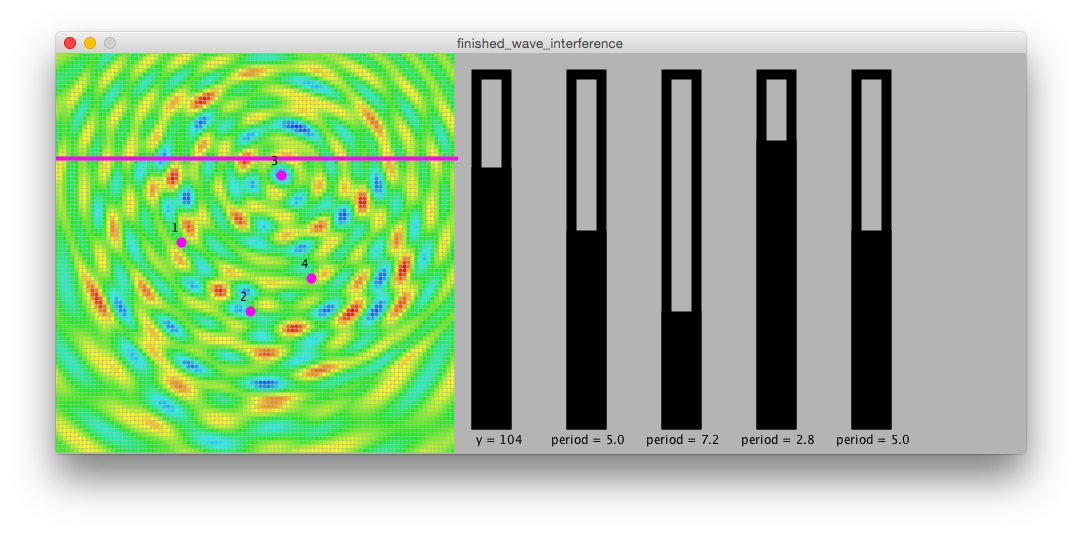
\includegraphics[width=\linewidth]{../result/4wave.png}
 \end{center}
 \caption{波の位相変位を視覚化したプログラムの画面.}
 \label{fig:4wave}
\end{figure}






\subsection{drawモード}
このモードは波源から生じる円形波を描写するモードである. プログラム起動時の画面が図\ref{fig:0wave}である.
\begin{figure}[htbp]
 \begin{center}
  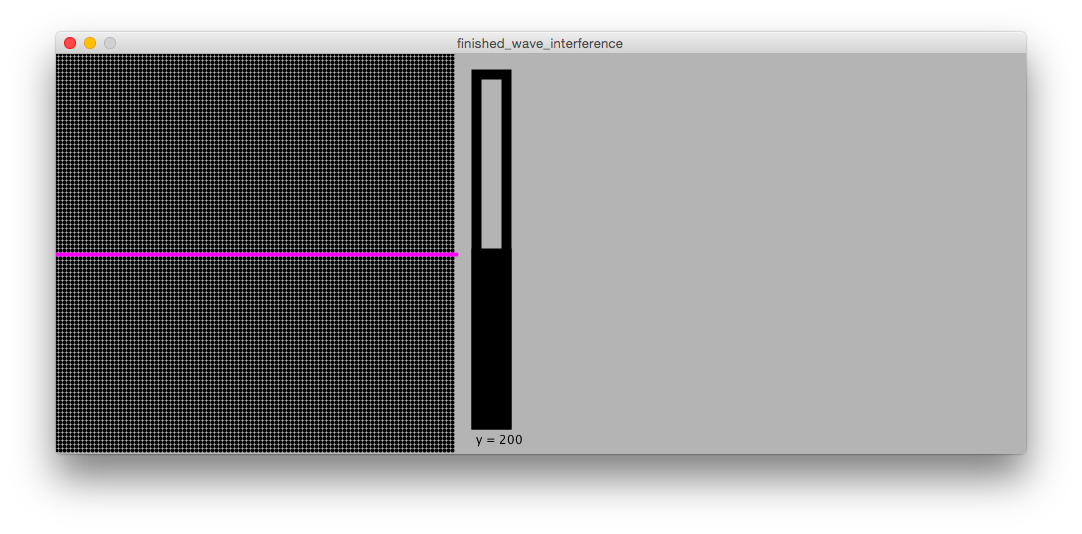
\includegraphics[width=\linewidth]{../result/0wave.png}
 \end{center}
 \caption{プログラム起動時の画面.}
 \label{fig:0wave}
\end{figure}

画面左側の黒い領域が波を描写する領域,画面右側にはcheckモードで確認するy座標の位置を操作できるスライダーが配置されている(いきなりスライダーと言っていいのか?). 
図\ref{fig:0wave}の状態で黒い領域上のいずれかの場所をクリックすると,クリックされた座標に波源が生成される.波源が生成されたあと,画面右側にはその波源の周期を変更できるスライダーが生成される.

図\ref{fig:wave}は1つの波源を生成した後,周期をスライダーによって変更した様子である.
\begin{figure}[htbp]
 \begin{center}
  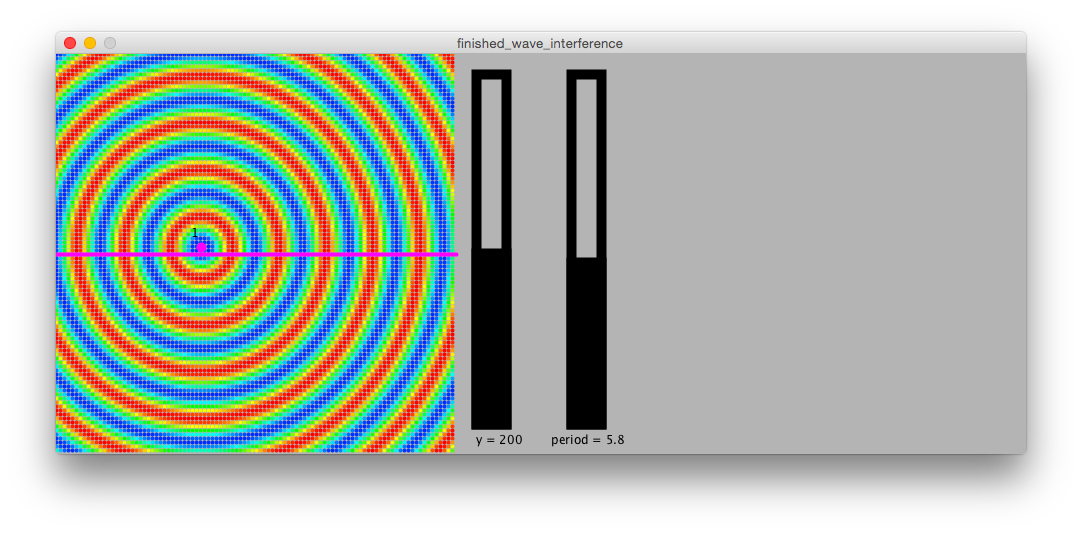
\includegraphics[width=\linewidth]{../result/wave.png}
 \end{center}
 \caption{1つの波の周期をスライダーで変更した画面.}
 \label{fig:wave}
\end{figure}

\newpage
スライダーが周期を変更できる状態で
Lキー(lambdaの頭文字)を押すと,図\ref{fig:wavechangelambda}のように波の波長を変更できるスライダーに変化する.周期を変更するスライダーに戻したい場合はPキー(periodの頭文字)を押せばよい.

\begin{figure}[htbp]
 \begin{center}
  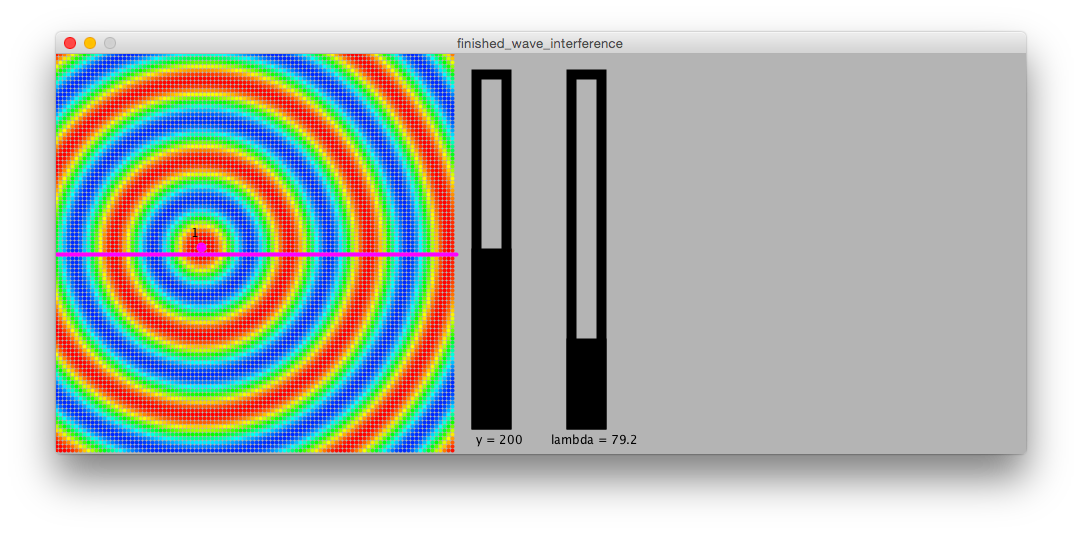
\includegraphics[width=\linewidth]{../result/wavechangelambda.png}
 \end{center}
 \caption{波長を変更できるスライダーに変化させた時の画面.}
 \label{fig:wavechangelambda}
\end{figure}

波源は図\ref{fig:5wave}のように5個まで生成できる.

\begin{figure}[htbp]
 \begin{center}
  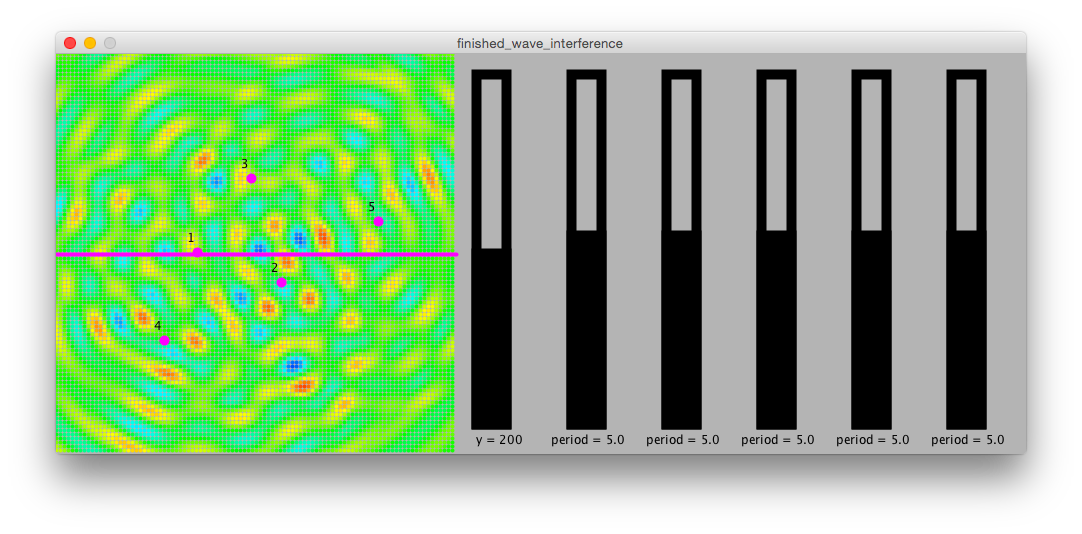
\includegraphics[width=\linewidth]{../result/5wave.png}
 \end{center}
 \caption{波源を5個生成した時の画面.}
 \label{fig:5wave}
\end{figure}

\newpage
\subsection{checkモード}
このモードはdrawモードに描写されている赤い線上の位相変位をリアルタイムに視覚化するモードである.同時刻,同座標で周期,波長が同一な波を生成し,波を生成して360フレーム目の状態をdrawモード,checkモードでそれぞれ描写したのが図\ref{fig:compare}(\subref{drawmode}),(\subref{checkmode})である.(ほんまに一致しているか先生に見てもらう)


\begin{figure}[htbp]
\begin{minipage}[b]{1.0\linewidth}
\centering
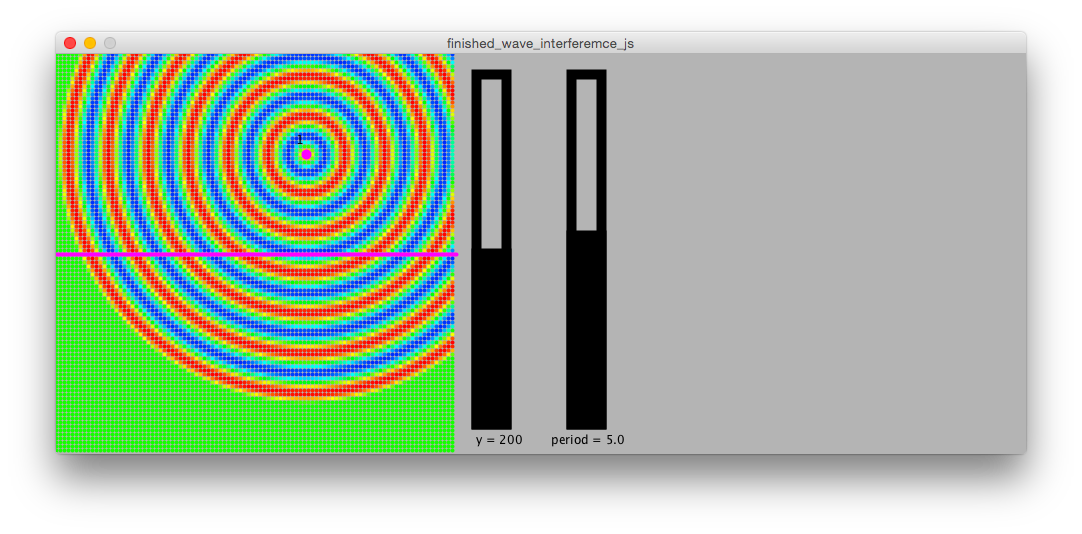
\includegraphics[keepaspectratio, scale=0.40]
  {../result/drawmode.png}
 \subcaption{drawモード.}\label{drawmode}
 \end{minipage}
 
\begin{minipage}[b]{1.0\linewidth}
\centering
  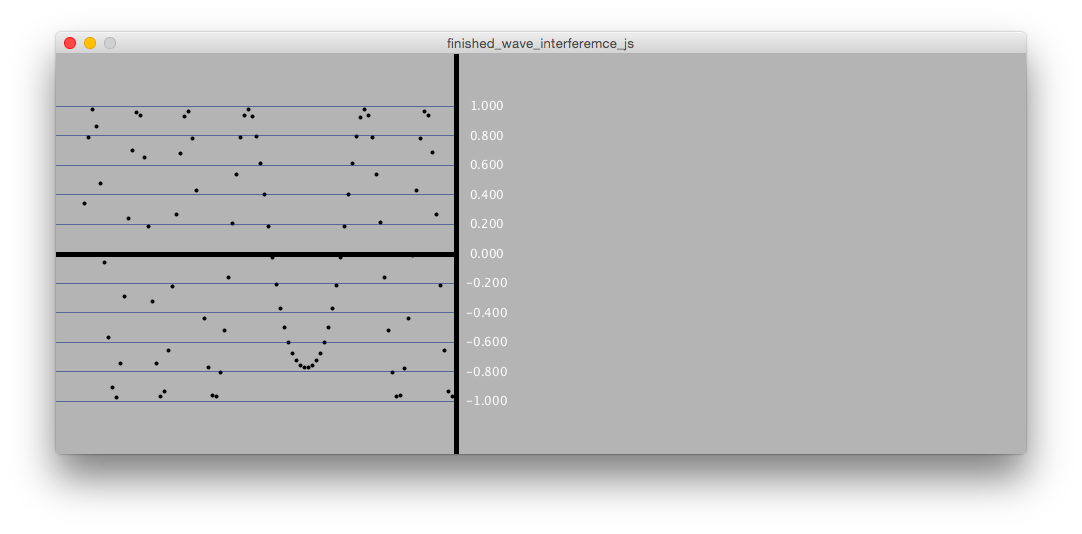
\includegraphics[keepaspectratio, scale=0.40]
  {../result/checkmode.png}
 \subcaption{checkモード.}\label{checkmode}
 \end{minipage}
  
  \caption{周期5.0,波長40.0の波が生成されてから360フレーム目のdrawモード,checkモードの画面.}
 \label{fig:compare}
\end{figure}



\newpage
\section{波の回折現象を視覚化したプログラム}
\section{波の反射を視覚化したプログラム}
出来なかった理由はプログラム解説の章で解説していいのか?
\section{波の屈折を視覚化したプログラム}























\begin{comment}

%図\ref{fig:MDprogram}は本研究で作成したVerlet法とLennard-Jonesポテンシャルを用いて粒子の振る舞いをシミュレーションし,視覚化を行うプログラムである.
%Processingで作成しているが,JavaScriptへ変換する事によってWebブラウザ上で動作させる事が可能である.
%左の枠内に複数の粒子モデルが描画され,それらが枠内を動き回る.また,粒子の色を速度によって青から赤に変化させてエネルギーの推移をわかりやすくし,マウスカーソルで粒子をクリックしドラッグする\input{result.tex}
%事によって好きな方向に力を加える事ができる.
%右側には2本のスライダーがあり,粒子の数とVerlet法の時間刻みを調整できる.
%キー入力により状態を変更することができ,Sキーで凝固状態,Fキーで粒子に加わる力を視覚化した状態,Rキーで粒子のリセットを行うことができる.

\newpage
\begin{figure}[htbp]
 \begin{center}
  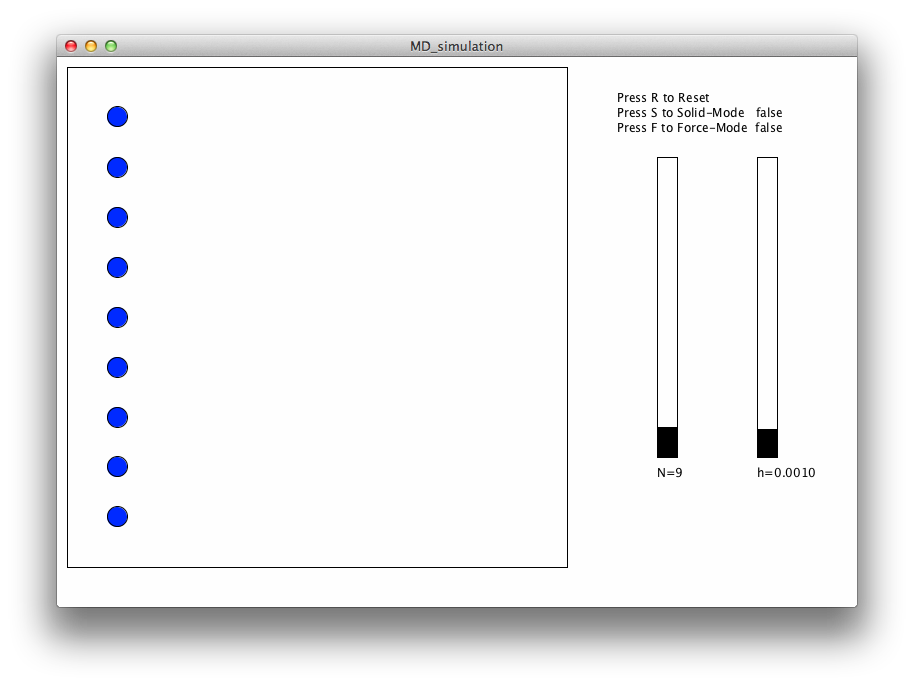
\includegraphics[width=150mm]{../implement/MDprogram.png} %implementのフォルダにあるpng画像
 \end{center}
 \caption{分子動力学法視覚化プログラム.}
 \label{fig:MDprogram}
\end{figure}

\newpage

図\ref{fig:cluster}は粒子クラスタの移動を表しており,それぞれの粒子のクラスタとしての振る舞いを視認することができる.
スライダーで粒子の数を変更しマウスで力を加えることによって,このようなクラスタを好きなようにシミュレーションできる.
\begin{figure}[htbp]
 \begin{center}
  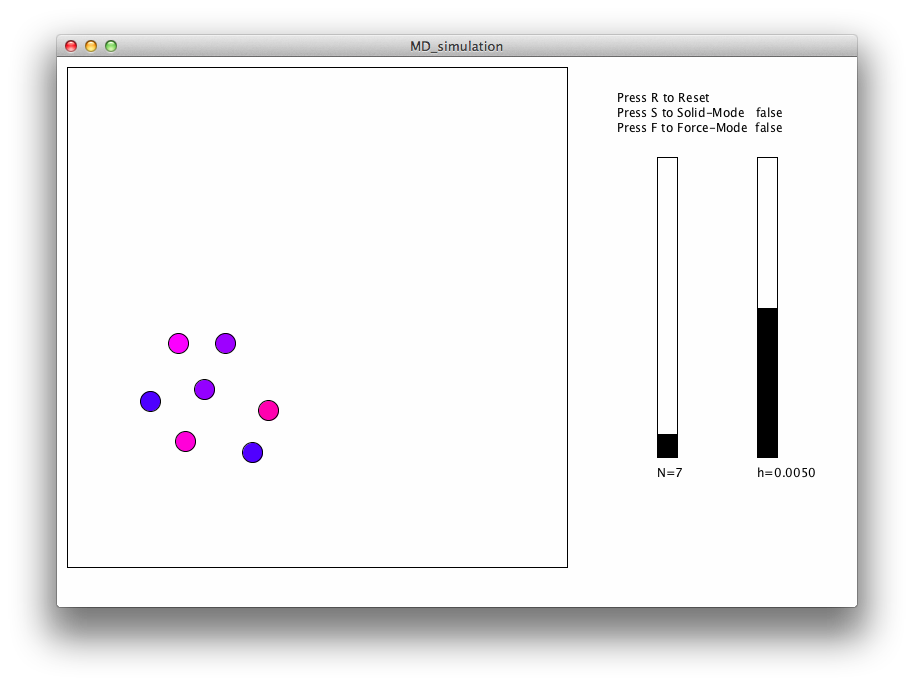
\includegraphics[width=150mm]{../result/cluster_picture.png}
 \end{center}
 \caption{クラスタの移動.}
 \label{fig:cluster}
\end{figure}


\newpage

図\ref{fig:solid}は凝固状態にしてしばらく実行し続けた結果であり,粒子が下の方に集まっていることが確認できる.これは粒子に下向きの力を継続的に加えて擬似的に凝固の現象を表現している.
これにより,粒子が自由に動き回る液体や気体の状態から,個体に移り変わる凝固現象の様子を確認できる.


\begin{figure}[htbp]
 \begin{center}
  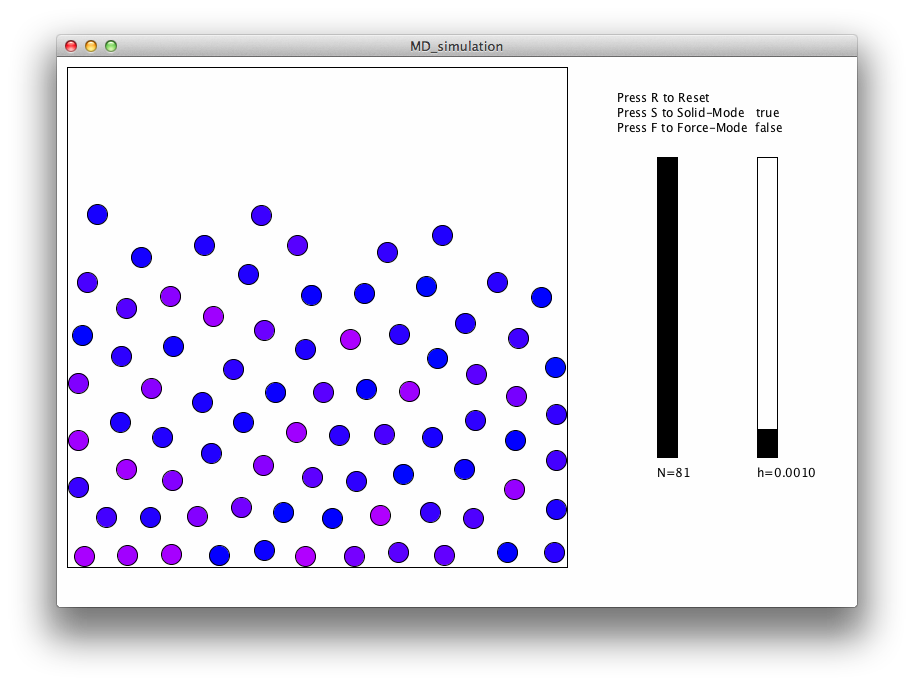
\includegraphics[width=150mm]{../implement/solid_mode.png}
 \end{center}
 \caption{凝固状態.}
 \label{fig:solid}
\end{figure}

\newpage

図\ref{fig:force}は粒子に加わる力を視覚化した状態であり,それぞれの粒子の中心から線が伸びている.
この線は長さが力の大きさ,向きが力の向きと対応しており力の加わり方をリアルタイムで把握することができる.
それぞれの粒子が力のパラメータを持っており,それらはシュミレーションの中で瞬時に変化していくため,値の確認は困難である.
しかし,この視覚化のおかげでそれぞれの粒子にかかる力を直感的に確認できる.

\begin{figure}[htbp]
 \begin{center}
  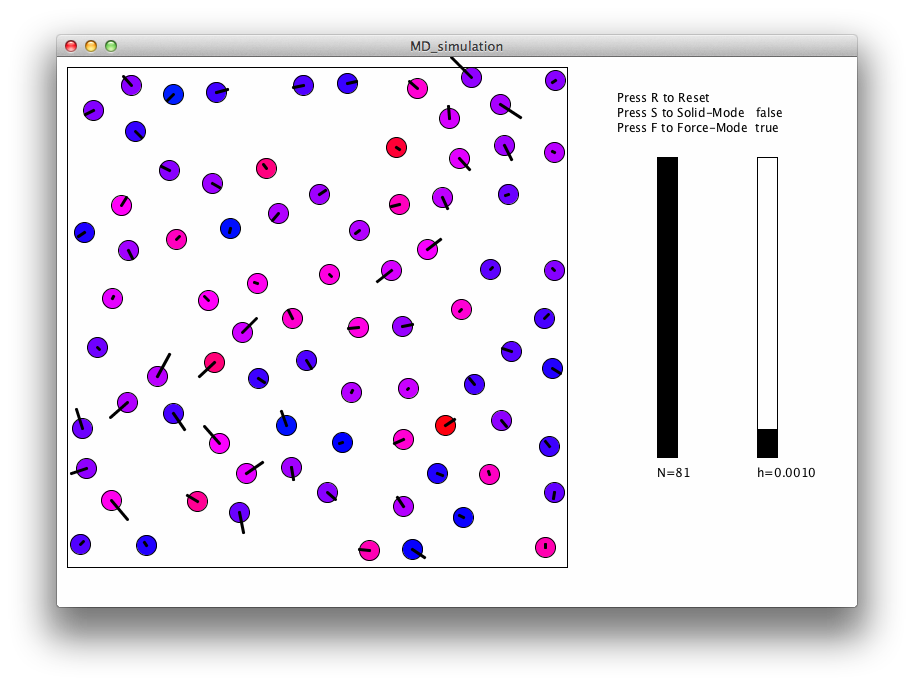
\includegraphics[width=150mm]{../implement/force_mode.png}
 \end{center}
 \caption{粒子に加わる力を視覚化した状態.}
 \label{fig:force}
\end{figure}


\end{comment}

%事によって好きな方向に力を加える事ができる.
%右側には2本のスライダーがあり,粒子の数とVerlet法の時間刻みを調整できる.
%キー入力により状態を変更することができ,Sキーで凝固状態,Fキーで粒子に加わる力を視覚化した状態,Rキーで粒子のリセットを行うことができる.

\newpage
\begin{figure}[htbp]
 \begin{center}
  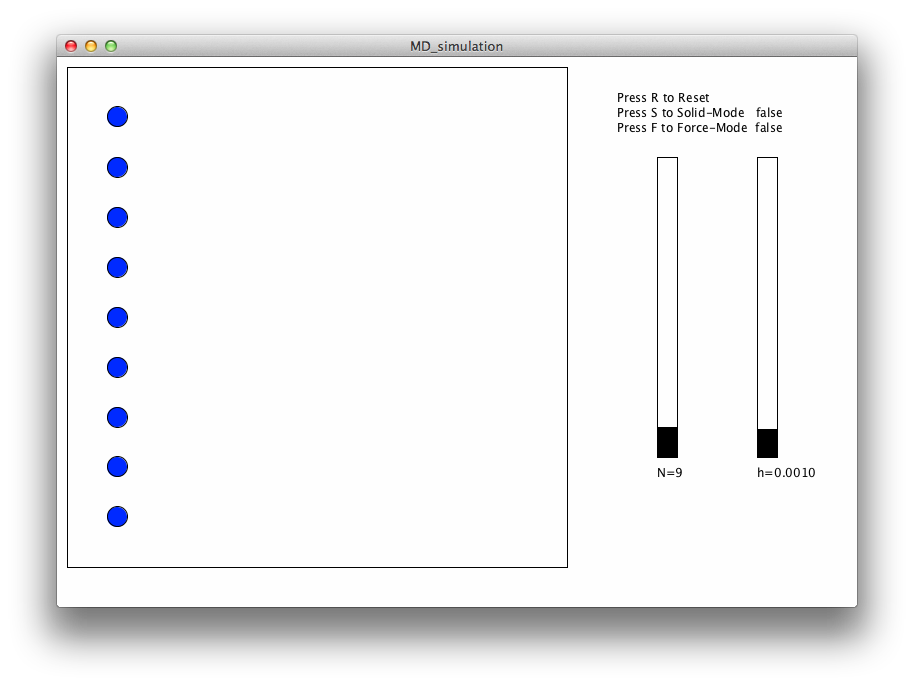
\includegraphics[width=150mm]{../implement/MDprogram.png} %implementのフォルダにあるpng画像
 \end{center}
 \caption{分子動力学法視覚化プログラム.}
 \label{fig:MDprogram}
\end{figure}

\newpage

図\ref{fig:cluster}は粒子クラスタの移動を表しており,それぞれの粒子のクラスタとしての振る舞いを視認することができる.
スライダーで粒子の数を変更しマウスで力を加えることによって,このようなクラスタを好きなようにシミュレーションできる.
\begin{figure}[htbp]
 \begin{center}
  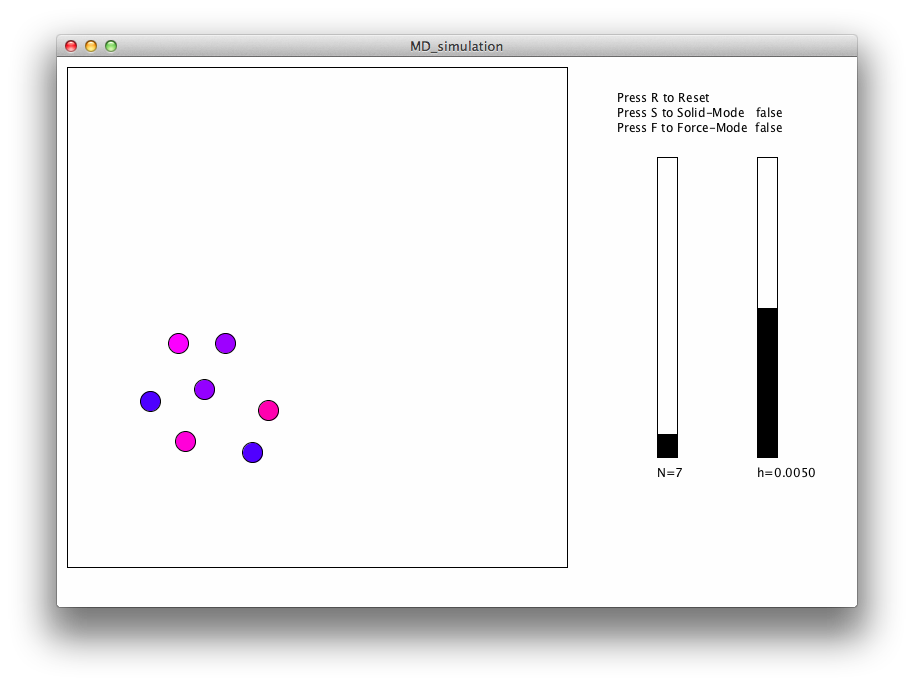
\includegraphics[width=150mm]{../result/cluster_picture.png}
 \end{center}
 \caption{クラスタの移動.}
 \label{fig:cluster}
\end{figure}


\newpage

図\ref{fig:solid}は凝固状態にしてしばらく実行し続けた結果であり,粒子が下の方に集まっていることが確認できる.これは粒子に下向きの力を継続的に加えて擬似的に凝固の現象を表現している.
これにより,粒子が自由に動き回る液体や気体の状態から,個体に移り変わる凝固現象の様子を確認できる.


\begin{figure}[htbp]
 \begin{center}
  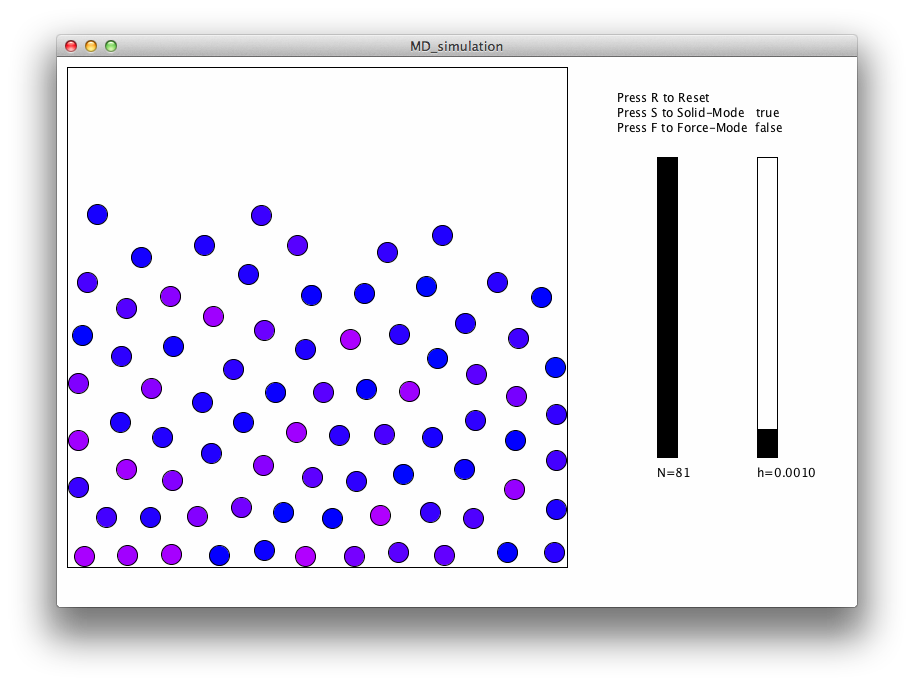
\includegraphics[width=150mm]{../implement/solid_mode.png}
 \end{center}
 \caption{凝固状態.}
 \label{fig:solid}
\end{figure}

\newpage

図\ref{fig:force}は粒子に加わる力を視覚化した状態であり,それぞれの粒子の中心から線が伸びている.
この線は長さが力の大きさ,向きが力の向きと対応しており力の加わり方をリアルタイムで把握することができる.
それぞれの粒子が力のパラメータを持っており,それらはシュミレーションの中で瞬時に変化していくため,値の確認は困難である.
しかし,この視覚化のおかげでそれぞれの粒子にかかる力を直感的に確認できる.

\begin{figure}[htbp]
 \begin{center}
  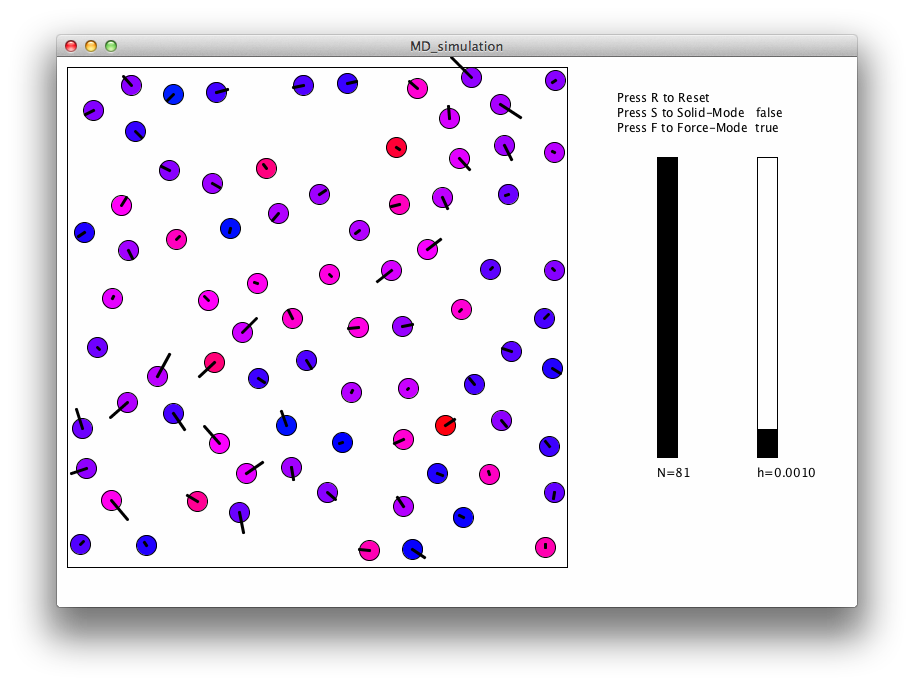
\includegraphics[width=150mm]{../implement/force_mode.png}
 \end{center}
 \caption{粒子に加わる力を視覚化した状態.}
 \label{fig:force}
\end{figure}


\end{comment}

%事によって好きな方向に力を加える事ができる.
%右側には2本のスライダーがあり,粒子の数とVerlet法の時間刻みを調整できる.
%キー入力により状態を変更することができ,Sキーで凝固状態,Fキーで粒子に加わる力を視覚化した状態,Rキーで粒子のリセットを行うことができる.

\newpage
\begin{figure}[htbp]
 \begin{center}
  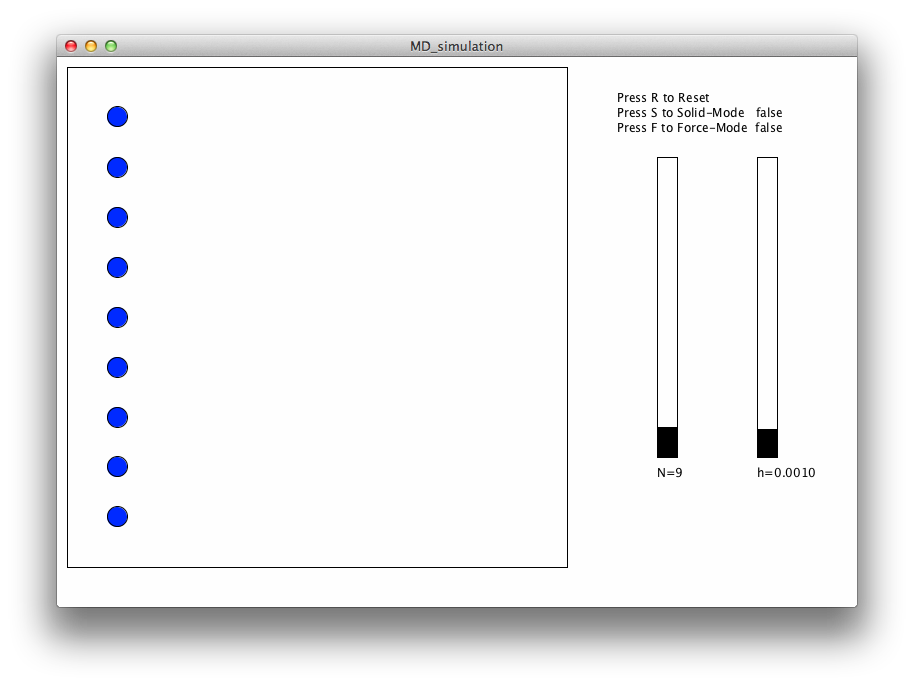
\includegraphics[width=150mm]{../implement/MDprogram.png} %implementのフォルダにあるpng画像
 \end{center}
 \caption{分子動力学法視覚化プログラム.}
 \label{fig:MDprogram}
\end{figure}

\newpage

図\ref{fig:cluster}は粒子クラスタの移動を表しており,それぞれの粒子のクラスタとしての振る舞いを視認することができる.
スライダーで粒子の数を変更しマウスで力を加えることによって,このようなクラスタを好きなようにシミュレーションできる.
\begin{figure}[htbp]
 \begin{center}
  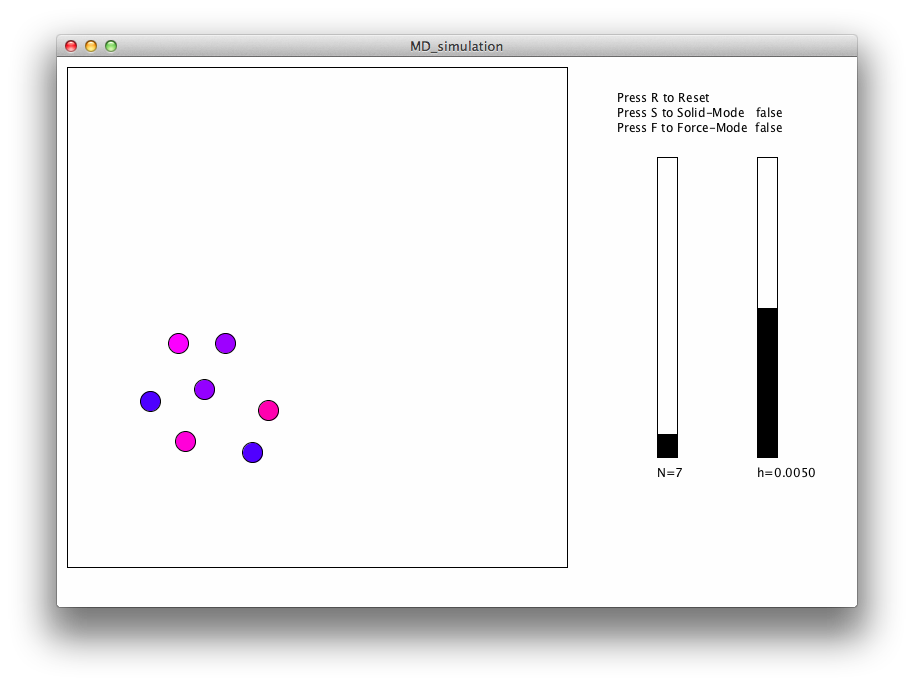
\includegraphics[width=150mm]{../result/cluster_picture.png}
 \end{center}
 \caption{クラスタの移動.}
 \label{fig:cluster}
\end{figure}


\newpage

図\ref{fig:solid}は凝固状態にしてしばらく実行し続けた結果であり,粒子が下の方に集まっていることが確認できる.これは粒子に下向きの力を継続的に加えて擬似的に凝固の現象を表現している.
これにより,粒子が自由に動き回る液体や気体の状態から,個体に移り変わる凝固現象の様子を確認できる.


\begin{figure}[htbp]
 \begin{center}
  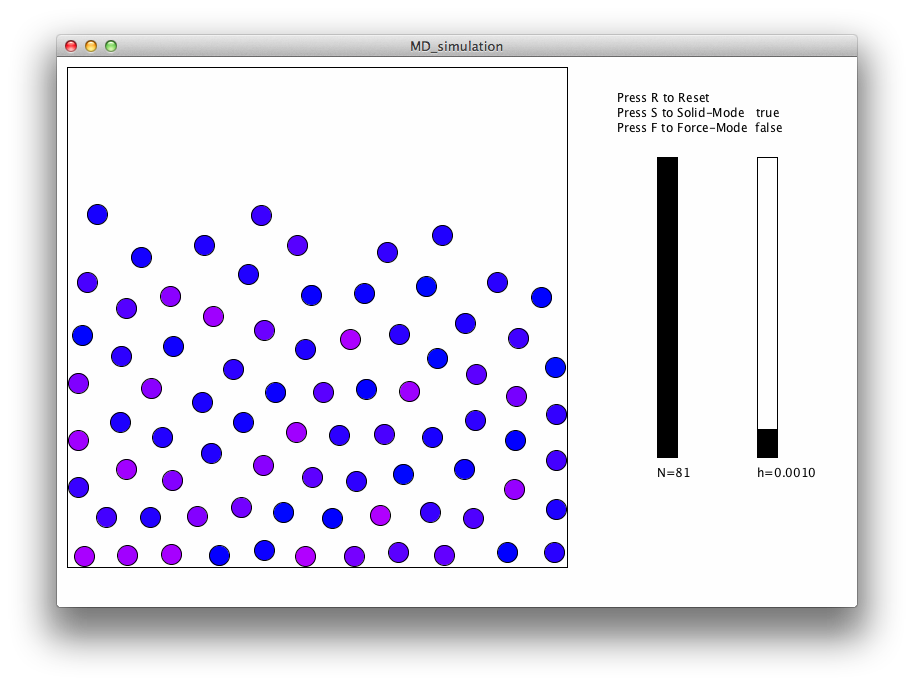
\includegraphics[width=150mm]{../implement/solid_mode.png}
 \end{center}
 \caption{凝固状態.}
 \label{fig:solid}
\end{figure}

\newpage

図\ref{fig:force}は粒子に加わる力を視覚化した状態であり,それぞれの粒子の中心から線が伸びている.
この線は長さが力の大きさ,向きが力の向きと対応しており力の加わり方をリアルタイムで把握することができる.
それぞれの粒子が力のパラメータを持っており,それらはシュミレーションの中で瞬時に変化していくため,値の確認は困難である.
しかし,この視覚化のおかげでそれぞれの粒子にかかる力を直感的に確認できる.

\begin{figure}[htbp]
 \begin{center}
  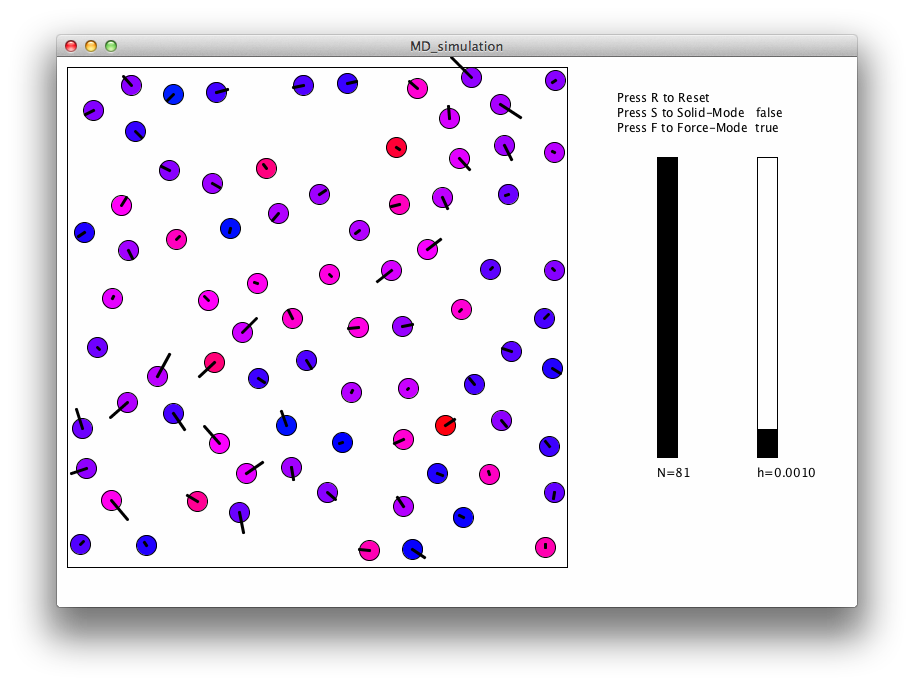
\includegraphics[width=150mm]{../implement/force_mode.png}
 \end{center}
 \caption{粒子に加わる力を視覚化した状態.}
 \label{fig:force}
\end{figure}


\end{comment}

%事によって好きな方向に力を加える事ができる.
%右側には2本のスライダーがあり,粒子の数とVerlet法の時間刻みを調整できる.
%キー入力により状態を変更することができ,Sキーで凝固状態,Fキーで粒子に加わる力を視覚化した状態,Rキーで粒子のリセットを行うことができる.

\newpage
\begin{figure}[htbp]
 \begin{center}
  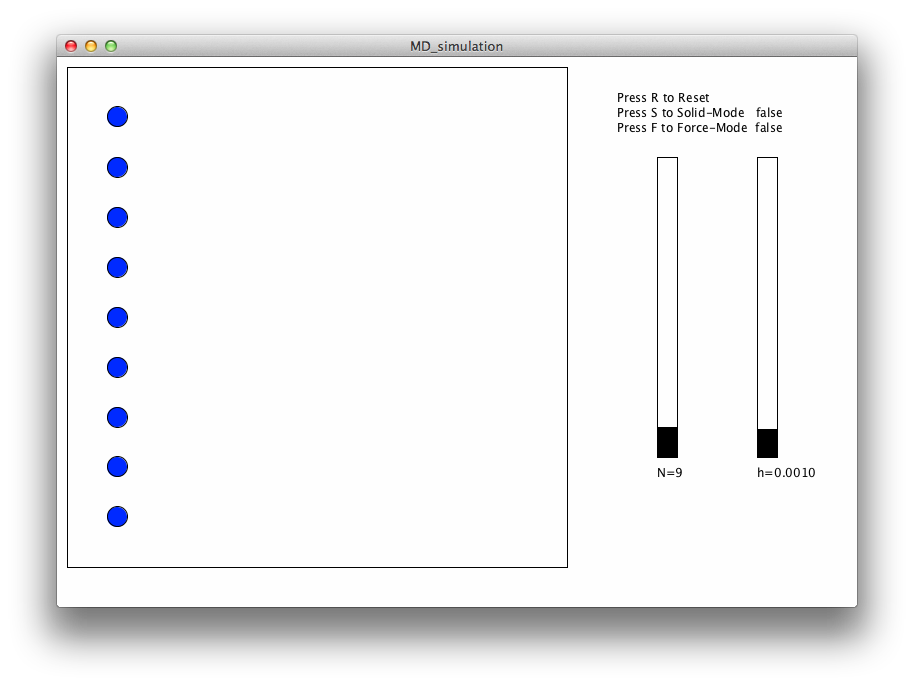
\includegraphics[width=150mm]{../implement/MDprogram.png} %implementのフォルダにあるpng画像
 \end{center}
 \caption{分子動力学法視覚化プログラム.}
 \label{fig:MDprogram}
\end{figure}

\newpage

図\ref{fig:cluster}は粒子クラスタの移動を表しており,それぞれの粒子のクラスタとしての振る舞いを視認することができる.
スライダーで粒子の数を変更しマウスで力を加えることによって,このようなクラスタを好きなようにシミュレーションできる.
\begin{figure}[htbp]
 \begin{center}
  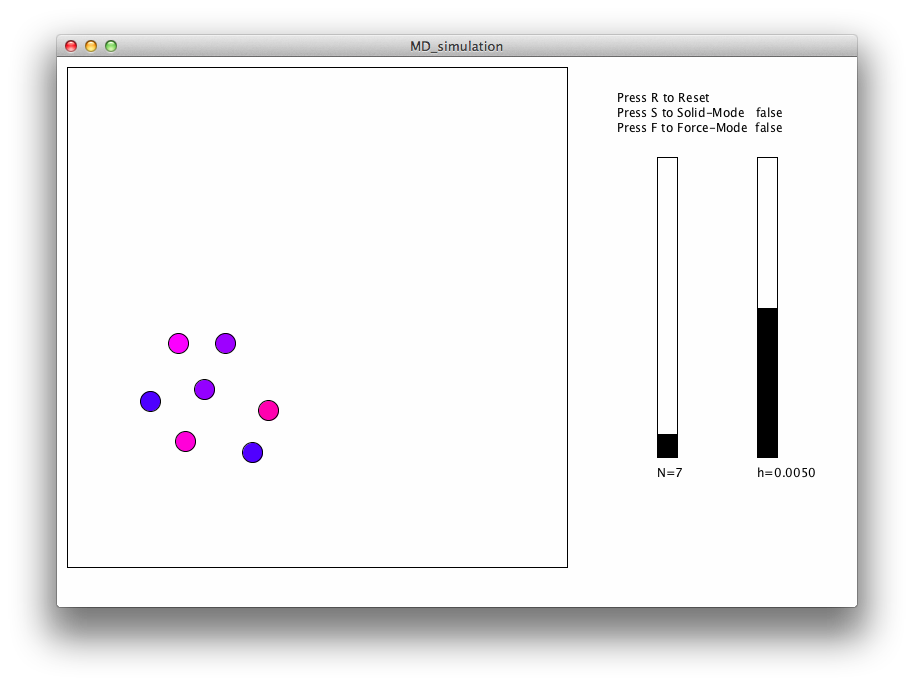
\includegraphics[width=150mm]{../result/cluster_picture.png}
 \end{center}
 \caption{クラスタの移動.}
 \label{fig:cluster}
\end{figure}


\newpage

図\ref{fig:solid}は凝固状態にしてしばらく実行し続けた結果であり,粒子が下の方に集まっていることが確認できる.これは粒子に下向きの力を継続的に加えて擬似的に凝固の現象を表現している.
これにより,粒子が自由に動き回る液体や気体の状態から,個体に移り変わる凝固現象の様子を確認できる.


\begin{figure}[htbp]
 \begin{center}
  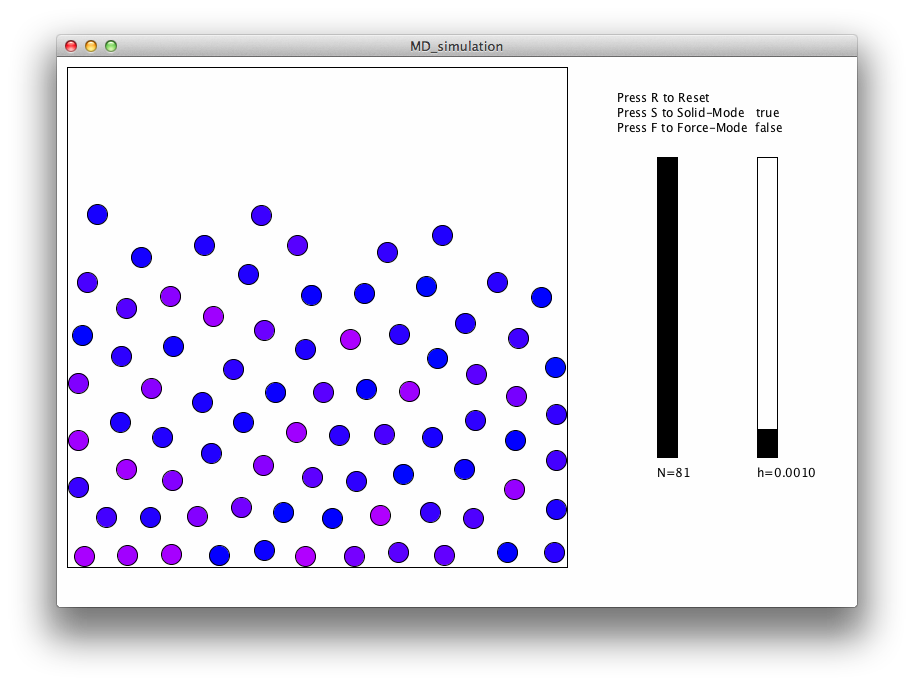
\includegraphics[width=150mm]{../implement/solid_mode.png}
 \end{center}
 \caption{凝固状態.}
 \label{fig:solid}
\end{figure}

\newpage

図\ref{fig:force}は粒子に加わる力を視覚化した状態であり,それぞれの粒子の中心から線が伸びている.
この線は長さが力の大きさ,向きが力の向きと対応しており力の加わり方をリアルタイムで把握することができる.
それぞれの粒子が力のパラメータを持っており,それらはシュミレーションの中で瞬時に変化していくため,値の確認は困難である.
しかし,この視覚化のおかげでそれぞれの粒子にかかる力を直感的に確認できる.

\begin{figure}[htbp]
 \begin{center}
  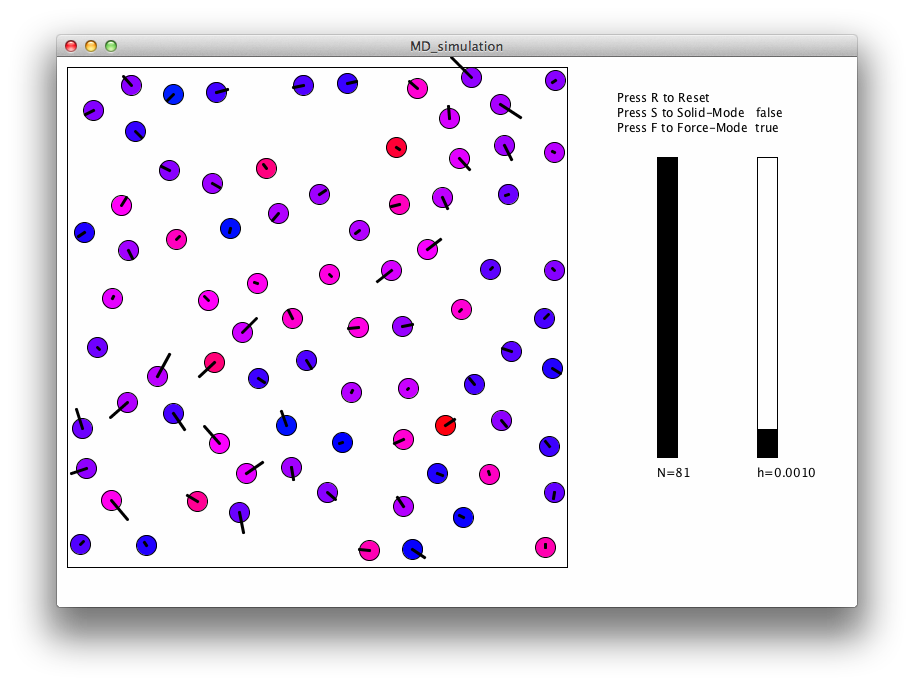
\includegraphics[width=150mm]{../implement/force_mode.png}
 \end{center}
 \caption{粒子に加わる力を視覚化した状態.}
 \label{fig:force}
\end{figure}


\end{comment}
